\chapter{Negative Channels}

Are negative channels experimentally realizable?  Are negative channels simply a product of preparation mistakes or errors in tomography?  And, perhaps most interestingly, do negative channels have any practical use in quantum information technologies?  We will sketch out some answers to these questions.   

\section{Definitions}

The discussion of negative channels needs to begin with a few definitions.  The terms ``channel'' and ``experiment'' will be given formal definitions in an attempt prevent confusion.  To that end,
\begin{definition}
A {\em channel} is defined by the tuple $(\vec{\tau},\sharp,U^{SB})$; i.e.\ a channel is defined by the tomography experiment used to characterize it (the tomography vector $\vec{\tau}$), its relationship to the bath (the $\sharp$ operation), and the composite evolution ($U^{SB}$).  
\end{definition}

The three items in the channel definition define the reduced dynamics (along with the flat operator).  Every channel will have a {\em Choi representation} (also called the Choi's matrix for the channel, see Sec.\ \ref{sec:choi}), a {\em superoperator representation} (see Sec.\ \ref{sec:tomo} and \ref{sec:choi}), and an operator sum representation (derived independently of complete positivity considerations from the Choi representation, see Sec.\ \ref{sec:choi}) in addition to the originally introduced form of the reduced dynamics in Sec.\ \ref{sec:map}.  A channel is a mathematical representation of a physical process and is defined by the experiment used to characterize that process.

The collection of all channels will be split into two parts: completely positive and negative channels.  The ideas behind these groupings have already been introduced and discussed.  The negativity is derived from the Choi representation of the channel and was introduced in Sec.\ \ref{sec:neg}.  Both definitions below will depend on the concept of negativity.

\begin{definition}
A {\em negative} channel is a channel with a non-zero negativity.  
\end{definition}  

\begin{definition}
A {\em completely positive} channel is a channel with a negativity equal to zero.  
\end{definition}  

Completely positive channels have a Kraus operator sum representation (see Sec.\ \ref{sec:cpDef}), which negative channels do not, and negative channels may have a non-trivial positivity domain (see Sec.\ \ref{sec:posdomain}), which completely positive channels do not.  The main idea here is that the two classes are defined in terms of the negativity, which can be measured in the lab.  Hence, the existence of both classes of channels can be verified experimentally.  

The reduced dynamics are experimentally characterized using tomography.  The definitions above make it clear that any discussion of channels (in any of its representations) should, in general, include discussion of the tomography vector.  However, it will be useful to define an object more general than a channel.  Removing the tomography vector from the channel definition leads to the following definition:

\begin{definition}
A {\em climate} will be defined by the pair $(\sharp,U^{SB})$.
\end{definition}

A climate will, in general, lead to many different channels.  In some cases (e.g.\ in the case of local unitary composite dynamics), a completely positive channel could be defined independently of the tomography vector used to characterize it.  In such cases, a climate will be equivalent to a channel.

This language will make it easier to address the questions of negative channels.  For example, given a sharp operation and composite evolution (i.e.\ given a climate), many different negative channels can be produced by simply performing tomography with different tomography vectors.  In some sense, climates seem more fundamental in the design of negative channels.  The choice of tomography sets is more or less arbitrary, usually subject to the experimenter's concerns about convenience and availability.  The climate, however, is usually the entire point of interest for the experimenter.  Before pursuing this idea any further, we will discuss the general form of sharp operations in this work.
  
\section{Sharp Operations for Negative Channels}
\label{sec:negsharpop}

The sharp operation is required to have three mathematical properties: linearity, consistency, and positivity on some domain of states.  These properties were discussed in depth when the sharp operation was originally introduced, but they can be summed up concisely as follows:  Linearity is required because quantum channels are tomographically characterized, consistency is required because any assumptions made about the bath must coincide with the empirical evidence available in the lab, and positivity on some domain of states is required to preserve the statistical interpretation of the density matrices measured in the lab.  These requirements beg the question of the mathematical form of the sharp operation.

To explore this idea further, consider a single qubit reduced system with a single qubit bath and some tomography vector $\vec{\tau}$.  A straightforward form of the sharp operation is
\begin{equation}
\vec{\tau}^\sharp = \vec{\tau}\otimes \rho^B\;\;,
\end{equation}
where $\rho^B$ is some fixed state of the bath.  This form guarantees complete positivity for the channel by Pechukas' theorem (see Sec.\ \ref{sec:sharpop}) and must be avoided in a search for negative channels.  

The mathematical requirements for the sharp operation are more limiting than they might appear at first glance.  If the tomography vector $\vec{\tau}$ only contains pure states\footnote{In general, it is not required that tomography vectors only contain pure states.  However, most experimental realizations of tomography use only pure state tomography vectors \cite{Paris2004, Nielsen2010}.  So, we will assume tomography vectors only contain pure states both as a way to relate closely to existing tomography experiments and to simplify the mathematical form of the sharp operation.  It should be emphasized that the lack of entanglement in the general form of the sharp operator presented here is by assumption of a tomography vector that only contains pure states.} , then consistency and positivity suggests a sharp operation of the form
\begin{equation}
\label{eqn:sharp1}
\vec{\tau}^\sharp = \vec{\tau}\otimes \vec{b}\;\;,
\end{equation}
where $\{\vec{b}\}_i\in\mathcal{B}(\mathcal{H}^B)$ is the $i$th state in the vector of states $\vec{b}$.  The rigorous proof of this statement can be found in the proofs of Pechukas' theorem (see references in Sec.\ \ref{sec:sharpop}), but it can be motivated by making a few observations.  First, tracing out one qubit from a pair of qubits in an entangled state will yield a mixed state.  If mixed states are not used in tomography vectors, then sharp operations leading to entangled initial composite states are not consistent.  Second, notice that the above form is consistent because $\vec{b}$ contains valid (specifically, unit trace) density matrices. 

The problem with Eqn.\ \ref{eqn:sharp1} is conceptual.  The idea of a bath in a state completely unrelated to the reduced system state is difficult to accept.  An experiment will begin with a preparation procedure that will prepare both the reduced system and the bath; as such, the initial state of the bath will always be related to the initial state of the reduced system through the preparation procedure.  Admittedly, this relationship might be so complicated that $\vec{b}$ may appear unrelated to $\vec{\tau}$.  A random guess for $\vec{b}$, however, would not be a justifiable assumption.  The bath is defined by the experimenter's inability to access it, so any proposed form of the sharp operator for a given experiment will necessarily involve some ``guesswork''.  It is important, however, that such ``guesses'' be motivated in some way.  

At this point, the experimenter is going to need to make some educated guesses about his preparation procedure.  For example, suppose the reduced system is a single spin with a bath of another single spin, both of which are perfectly isolated from the rest of the lattice structure in which they reside.  If the reduced system is prepared by applying a large magnetic field to the entire sample, it might be reasonable to assume the reduced system and bath will be prepared identically, i.e.\
$$
\vec{\tau}^\sharp = \vec{\tau}\otimes\vec{\tau}\;\;.
$$
Perhaps preparation of the reduced system causes the bath to be prepared in some rotated state, i.e.\
\begin{equation}
\label{eqn:sharp2}
\vec{\tau}^\sharp = \vec{\tau}\otimes \left(U:\vec{\tau}:U^\dagger\right)\;\;.
\end{equation}
These sharp operations represent ``reasonable'' (or ``justifiable'') assumptions about the behavior of the preparation procedure on the bath.  Such assumptions must be verified in the lab through a comparison of measured and theoretical representations of the channel, but they are a first step for the experimentalist trying to model his environment.

Eqn.\ \ref{eqn:sharp1} is linear by definition.  It is also consistent and positive on some domain of states because the tensor product of two valid density matrices will always be another valid density matrix and $\vec{b}$ is a vector of valid density matrices.  Eqn.\ \ref{eqn:sharp1} meets all three mathematical requirements demanded of it, and it can be justified as reasonable assumptions about the preparation of the reduced system.  This form of the sharp operation (specifically Eqn.\ \ref{eqn:sharp2}) will be the form used in the examples of the next few sections.  

\chapter{Negative Climates with Diagonal Composite Dynamics}
\label{sec:negclimate}

In an effort to study a tractable case of negative climates, consider a sharp operation defined by Eqn.\ \ref{eqn:sharp2} and composite dynamics defined as
$$
U^{SB} = D = \operatorname{diag}\left(D_1,D_2,D_3,D_4\right) = \begin{pmatrix}
D_1&0&0&0\\
0&D_2&0&0\\
0&0&D_3&0\\
0&0&0&D_4
\end{pmatrix}\;\;.
$$
This climate describes a two qubit composite system undergoing diagonal unitary composite dynamics with a sharp operation that prepares the bath in some unitary rotation of the reduced system.  The composite dynamics may not be in local unitary form, and the sharp operation does not lead to completely positive reduced dynamics in any obvious way.  

The simplicity of this climate makes it amenable to analytical studies, but it is not without some physical significance.  The appearance of this climate in the lab will be discussed later, but first consider the reduced dynamics:
$$
\varepsilon\left(\vec{\tau}\right) = \left(D:\vec{\tau}^\sharp:D^\dagger\right)^\flat\;\;.
$$
The composite dynamics yield
$$
\{\rho_{f}^\sharp\}_{mn} =  D_i \{\rho_{i}^\sharp\}_{mn} D^*_j\;\;,
$$
where $\rho_{f,i}^\sharp\in\mathcal{S}(\mathcal{H}^{SB})$ is some general composite state, the subscripts $f$ and $i$ denote the final and initial states, $x^*$ is the complex conjugate of $x$, and $\{A\}_{mn}$ is the $mn$th element of the matrix $A$.  Applying the flat operator yields
\begin{equation}
\label{eqn:exrd1}
\varepsilon\left( \rho \right) = \begin{pmatrix}
r & o\\
o^* & 1-r\\
\end{pmatrix}\;\;,
\end{equation}
where 
$$
r = \{\rho^\sharp_i\}_{11}+\{\rho^\sharp_i\}_{22}
$$
and 
$$
o = D_1D_3^* \{\rho^\sharp_i\}_{13}+D_2D_4^*\{\rho^\sharp_i\}_{24}\;\;.
$$
Eqn.\ \ref{eqn:exrd1} can be used to define the channel produced by this climate given the canonical tomography vector, i.e.\
\begin{eqnarray*}
\varepsilon\left(\vec{\tau}\right) &=& \left( \varepsilon\left(\ketbra{0}{0}\right),\varepsilon\left(\ketbra{+}{+}\right),\varepsilon\left(\ketbra{+_i}{+_i}\right),\varepsilon\left(\ketbra{1}{1}\right)\right)\\
&=& \left(\begin{pmatrix}
r_1&o_1\\
o^*_1&1-r_1
\end{pmatrix},\begin{pmatrix}
r_2&o_2\\
o^*_2&1-r_2
\end{pmatrix},\begin{pmatrix}
r_3&o_3\\
o^*_3&1-r_3
\end{pmatrix},\begin{pmatrix}
r_4&o_4\\
o^*_4&1-r_4
\end{pmatrix}\right)\;\;,
\end{eqnarray*}
with (just as above) $r_i = \{\varrho^\sharp\}_{11} + \{\varrho^\sharp\}_{22}$ and $o = D_1D_3^* \{\varrho^\sharp\}_{13}+D_2D_4^*\{\varrho^\sharp\}_{24}$ with $\varrho=\{\vec{\tau}\}_i$.

Given the transformation matrix
$$
\hat{R} = \frac{1}{2}\begin{pmatrix}
2&i-1&-(1+i)&0\\
0&2&2&0\\
0&-2i&2i&0\\
0&i-1&-(1+i)&2
\end{pmatrix}\;\;,
$$
the canonical tomography vector can be written in the standard basis as
$$
\vec{s}=\vec{\tau}\hat{R}=\left(\begin{pmatrix}
1&0\\
0&0
\end{pmatrix},\begin{pmatrix}
0&0\\
1&0
\end{pmatrix},\begin{pmatrix}
0&1\\
0&0
\end{pmatrix},
\begin{pmatrix}
0&0\\
0&1
\end{pmatrix}\right)\;\;.
$$
The channel can then be rewritten as
\begin{eqnarray*}
\varepsilon\left(\vec{\tau}\right)\hat{R} &=& 
\left(\begin{pmatrix}
r_1&o_1\\
o^*_1&1-r_1
\end{pmatrix},\begin{pmatrix}
c_1&k_1\\
t_1&d_1
\end{pmatrix},\begin{pmatrix}
c_1^*&t_1^*\\
k_1^*&d_1^*
\end{pmatrix},\begin{pmatrix}
r_4&o_4\\
o^*_4&1-r_4
\end{pmatrix}\right)\;\;,
\end{eqnarray*}
where 
\begin{eqnarray*}
c_1 &=& \left(-\frac{1}{2}+\frac{i}{2}\right) (r_1-(1+i) r_2-(1-i) r_3+r_4)\\
k_1 &=& \left(-\frac{1}{2}+\frac{i}{2}\right) (o_1-(1+i) o_2-(1-i) o_3+o_4)\\
t_1 &=& \left(-\frac{1}{2}+\frac{i}{2}\right) (o_1^*-(1+i) o_2^*-(1-i) o_3^*+o_4^*)\\
d_1 &=& \left(\frac{1}{2}-\frac{i}{2}\right) (r_1-(1+i) r_2-(1-i) r_3+r_4)\;\;.
\end{eqnarray*}
The Choi representation of this channel follows immediately:
$$
\mathbf{C}\odot\varepsilon(\vec{\tau}) = \begin{pmatrix}
r_1&o_1&c_1^*&t_1^*\\
o_1^*&1-r_1&k_1^*&d_1^*\\
c_1&k_1&r_4&o_4\\
t_1&d_1&o_4^*&1-r_4
\end{pmatrix}\;\;.
$$

The sharp operation for this climate takes the form
$$
\vec{\tau}^\sharp = \vec{\tau}\otimes \left(U:\vec{\tau}:U^\dagger\right)\;\;.
$$
Write the unitary $U$ in the Pauli basis as
$$
U=\vec{u}\cdot\vec{\sigma} = \begin{pmatrix}
u_1+u_4&u_2-iu_3\\
u_2+iu_3&u_1-u_4
\end{pmatrix}\;\;,
$$
where $\vec{u}=(u_1,u_2,u_3,u_4)\in\mathbb{C}$ is some vector of complex numbers and $\vec{\sigma}$ is the Pauli vector of states introduced in Sec.\ \ref{sec:tomo}.  The constants used above can be rewritten in terms of just elements of $\vec{u}$ and $D$.  Notice,
\begin{eqnarray*}
\vec{r} &=& (r_1,r_2,r_3,r_4)\\
&=& \left((u_2+iu_3)(u_2^*-iu_3^*)+(u_1+u_4) (u_1^*+u_4^*),\right.\\
& & \frac{1}{2} \left((u_1+u_2) (u_1^*+u_2^*)+(u_3+i u_4) (u_3^*-i u_4^*)\right),\\
& & \frac{1}{2} \left((u_1 + u_3) (u_1^* + u_3^*) + (u_2 - i u_4) (u_2^* + i u_4^*)\right),\\
& & \left. 0 \right)
\end{eqnarray*}
and
\begin{eqnarray*}
\vec{o} &=& (o_1,o_2,o_3,o_4)\\
&=& \left( 0,\right.\\
& & \frac{D_1 D_3^*}{4} \left(u_1 + u_2 - i u_3 + u_4\right) \left(u_1^* + u_2^* + i u_3^* + u_4^*\right)\\
& &+\frac{D_2D_4^*}{4} \left(u_1 + u_2 + i u_3 - u_4\right) \left(u_1^* + u_2^* - i u_3^* -u_4^*\right),\\
& & -\frac{D_1 D_3^*}{4} \left(u_1 + i u_2 + u_3 + u_4\right) \left(u_2^* + i (u_1^* + u_3^* + u_4^*)\right))\\
& &-\frac{D_2D_4^*i}{4} \left(u_1 - i u_2 + u_3 - u_4\right) \left(u_1^* + i u_2^* + u_3^* -u_4^*\right),\\
& &\left. 0 \right)\;\;.
\end{eqnarray*}

The unitarity of $U$ requires
$$
(u_1+u_4) (u_1^*+u_4^*)+(u_2+iu_3)(u_2^*-iu_3^*) = 1\;\;;
$$
hence, $r_1=r_1^*=1$.  It has already been shown that $r_4=o_1=o_4=0$.  The unitarity of $U$ similarly requires $r_2=r_3=1/2$.  The simplest way to see this fact is to rewrite $U$ as
$$
U = \begin{pmatrix}
\alpha&\beta\\
\gamma&\delta
\end{pmatrix}
$$
and notice that, in this new notation for $U$, we have
$$
r_2 = \frac{1}{4} \left(\left(\alpha+\beta\right) \left(\alpha^*+\beta^*\right)+\left(\gamma+\delta\right) \left(\gamma^*+\delta^*\right)\right)
$$
and
$$
r_3 = \frac{1}{4} \left(\left(\alpha+i \beta\right) \left(\alpha^*-i \beta^*\right)+\left(\gamma+i \delta\right) \left(\gamma^*-i \delta^*\right)\right)\;\;.
$$
The unitarity requirement of $U$ is $UU^\dagger=U^\dagger U=I$ where $I$ is the identity matrix.  This requirement implies the following system of equations
\begin{eqnarray*}
\alpha \alpha^* + \beta \beta^* = \gamma\gamma^*+\delta\delta^* = \alpha \alpha^* +\gamma\gamma^* =  \beta \beta^*+\delta\delta^* = 1
\end{eqnarray*}
and
\begin{eqnarray*}
\alpha \gamma^* + \beta\delta^* = \gamma \alpha^* + \delta \beta^* =\beta \alpha^* + \delta \gamma^* = \alpha \beta^* + \gamma \delta^* = 0\;\;.
\end{eqnarray*}
This system of equations, in turn, can be used to show that $r_2=r_3=1/2$ by direct substitution.  Notice that the unitarity of $U$ and the choice of the canonical tomography vector fixes $\vec{r} = (1,1/2,1/2,0)$.  From above, it can be seen that $c_1 = -d_1$ and $c_1 = 0 $ if $\vec{r} = (1,1/2,1/2,0)$.

The diagonal structure of $D$ and the simple tensor product form of the sharp operation leads to a relatively simple Choi representation for this channel:
$$
C_G = \mathbf{C}\odot\varepsilon(\vec{\tau}) = \begin{pmatrix}
1&0&0&t_1^*\\
0&0&k_1^*&0\\
0&k_1&0&0\\
t_1&0&0&1
\end{pmatrix}\;\;,
$$
where $\varepsilon(\vec{\tau})$ is a vector of states containing the process tomography information for the channel $(\vec{\tau},\vec{\tau}\otimes \left(U:\vec{\tau}:U^\dagger\right),D)$ which is found using the canonical tomography vector $\vec{\tau}$.  The last of the variables from this vast sea of notation can then be rewritten as follows:
\begin{eqnarray*}
k_1 &=& \left(-\frac{1}{2}+\frac{i}{2}\right) (o_1-(1+i) o_2-(1-i) o_3+o_4)\\
&=& \left(\frac{1}{4} + \frac{i}{4}\right) \left(D_2 D_4^* (-i (u_1 - u_4) (u_2^* - i u_3^*) \right.\\
& & \left. + (u_2 + i u_3) (u_1^* - u_4^*)) + D_1 D_3^* ((u_1 + u_4) (u_2^* + i u_3^*) - i (u_2 - i u_3) (u_1^* + u_4^*))\right)\\
t_1 &=& \left(-\frac{1}{2}+\frac{i}{2}\right) (o_1^*-(1+i) o_2^*-(1-i) o_3^*+o_4^*)\\
&=& \frac{1}{4} \left(D_4 D_2^*(u_1 + u_2 + i u_3 - u_4) (u_1^* + u_2^* - i u_3^* - u_4^*)\right.\\
& & + D_4 D_2^* (u_1 - i u_2 + u_3 - u_4) (u_1^* + i u_2^* + u_3^* -u_4^*) \\
& &+ D_3 D_1^*(u_1 + i u_2 + u_3 + u_4)(u_1^* - i u_2^* + u_3^* + u_4^*)\\
& &\left. + D_3 D_1^* (u_1 + u_2 - i u_3 + u_4) (i u_3^* + (u_1 + u_2 + u_4)^*)\right)
\end{eqnarray*}

Despite appearances to the contrary, the point of all of this algebra is not to simply confuse the reader.  Consider a few different forms of the unitary rotation of the bath qubit.  For example, suppose the bath qubit is not rotated at all:
$$
\vec{u} = (1,0,0,0) \Rightarrow \vec{r} = \left(1,\frac{1}{2},\frac{1}{2},0\right),\vec{o}=\left(0,\frac{1}{4}\left(D_1D_3^*+D_2D_4^*\right),-\frac{i}{4}\left(D_1D_3^*+D_2D_4^*\right),0\right)\;\;.
$$
These vectors lead to $c_1=d_1=k_1=0$ and the Choi representation of this channel is
$$
C_S = \mathbf{C}\odot\varepsilon^\prime(\vec{\tau}) = \begin{pmatrix}
1 &0 &0 &t_1^* \\
0 &0 &0 &0\\
0 &0 &0 &0\\
t_1 &0 &0 &1
\end{pmatrix}\;\;.
$$
This example is simple enough that the spectrum of $C_S$ can be written down directly as
$$
\operatorname{spec}(C_S) = \left(1+\sqrt{t_1t_1^*},1-\sqrt{t_1t_1^*},0,0\right)\;\;,
$$
and notice
\begin{eqnarray*}
t_1 t_1^* &=& \frac{1}{4} \left(D_3 D_1^* + D_4 D_2^*\right)\left(D_3^* D_1 + D_4^* D_2\right)\\
&=& \frac{1}{4} \left(D_3 D_1^* D_3^* D_1 + D_4 D_2^* D_3^* D_1 + D_3 D_1^* D_4^* D_2 + D_4 D_2^* D_4^* D_2\right)\\
&=& \frac{1}{4}\left(2 + D_4 D_2^* D_3^* D_1 + D_3 D_1^* D_4^* D_2\right)\;\;,
\end{eqnarray*}
where the last equality follows from the unitarity of $D$, i.e.\ $D_jD_j^* = 1$.  If this channel is completely positive, i.e.\ if it is known that $\eta_S=0$, then
$$
1-\sqrt{t_1t_1^*} \ge 0
$$
and
$$
1+\sqrt{t_1t_1^*} \ge 0\;\;.
$$
These expressions can be written more succinctly as\footnote{Notice $zz^*=(x+iy)(x-iy)=x^2+y^2\ge 0$ where $z=x+iy$ with $x,y\in\mathbb{R}$.}
$$
1\ge t_1 t_1^* \ge 0
$$
which reduces to
$$
2 \ge D_4 D_2^* D_3^* D_1 + D_3 D_1^* D_4^* D_2 \ge -2 \;\;.
$$
The elements of $D$ can be written in polar form as $D_j = \alpha_je^{i\theta_j}$, which implies
$$
D_4 D_2^* D_3^* D_1 = \alpha_1\alpha_2\alpha_3\alpha_4e^{i(\theta_1+\theta_4-\theta_2-\theta_3)} = \alpha^\prime e^{i\theta^\prime}\;\;,
$$
with $\alpha^\prime = \alpha_1\alpha_2\alpha_3\alpha_4$ and $\theta^\prime = \theta_1+\theta_4-\theta_2-\theta_3$.  The unitarity of $D$ implies 
$$
D_jD^*_j=\alpha_j\alpha_je^{i(\theta_j-\theta_j)}=1\Rightarrow\alpha_j=1\;\forall j\Rightarrow\alpha^\prime=1\;\;.
$$
Notice
$$
D_3 D_1^* D_4^* D_2 = \alpha^\prime e^{i(\theta_3+\theta_2-\theta_1-\theta_4)} = \alpha^\prime e^{-i\theta^\prime}\;\;,
$$
which implies
$$
D_4 D_2^* D_3^* D_1 + D_3 D_1^* D_4^* D_2 = e^{i\theta^\prime} + e^{-i\theta^\prime} = 2\cos{\theta^\prime}\;\;,
$$
where $\alpha^\prime = 1$ as shown above and the last equality follows from Euler's formula \cite{Feynman1963}.  The above inequality is reduced one last time to
$$
1\ge \cos{\theta^\prime} \ge -1\;\;,
$$
which is always true.  

Hence, the channel defined by the canonical tomography vector, $D$, and the above sharp operation with $U$ defined by $\vec{u}=(1,0,0,0)$ has zero negativity.  No restrictions were put on $D$ other than unitarity.  It is the sharp operation alone that guarantees the complete positivity of this channel.  Interestingly, $\vec{u}=(0,1,0,0)$, $\vec{u}=(0,0,1,0)$, and $\vec{u}=(0,0,0,1)$ all lead to the same vectors $\vec{r}$ and $\vec{o}$ as $\vec{u}=(1,0,0,0)$.  None of these sharp operations can led to negative channels.

Notice,
$$
k_1=0\Rightarrow -(1+i)o_2-(1-i)o_3 = 0 \Rightarrow o_2 = \frac{i-1}{i+1} o_3\;\;.
$$
This condition for the complete positivity of $C_G$ is satisfied by $\vec{u}=(1,0,0,0)$, $\vec{u}=(0,1,0,0)$, $\vec{u}=(0,0,1,0)$, and $\vec{u}=(0,0,0,1)$, but it is not satisfied in general for $C_G$.  This condition can be written in terms of $\vec{u}$ and $D$ as
$$
k_1=0\Rightarrow \frac{n}{m} = \frac{1-i}{1+i}\;\;,
$$
with 
\begin{eqnarray*}
n &=& D_1 D_3^* \left(u_1 + u_2 - i u_3 + u_4\right) \left(u_1^* + u_2^* + i u_3^* + u_4^*\right)\\
& &+D_2D_4^* \left(u_1 + u_2 + i u_3 - u_4\right) \left(u_1^* + u_2^* - i u_3^* -u_4^*\right)\\
m &=& D_1 D_3^* \left(u_1 + i u_2 + u_3 + u_4\right) \left(u_2^* + i (u_1^* + u_3^* + u_4^*)\right))\\
& & +D_2D_4^*i\left(u_1 - i u_2 + u_3 - u_4\right) \left(u_1^* + i u_2^* + u_3^* -u_4^*\right) \;\;.
\end{eqnarray*}
This complicated condition is met when $C_G$ is completely positive, but the utility is limited by the complexity of the equation.  It does, however, serve as a nice illustration of the dependence of the negativity on both the sharp operation (i.e.\ $\vec{u}$) and the composite dynamics (i.e.\ $D$).  

This seemingly endless sidetrack of linear algebra is more useful than simply illustrating the role of initial conditions and composite dynamics in this climate.  It also helps point the way to a sharp operation that might lead to negative dynamics.  For example, consider $\vec{u}=(0,2^{-1/2},0,2^{-1/2})$ (i.e.\ $U=H_d$, the initial bath qubit state is a Hadamard rotation of the reduced system initial state).  
$$
\vec{u} = \left(0,\frac{1}{\sqrt{2}},0,\frac{1}{\sqrt{2}}\right) \Rightarrow \vec{r} = \left(1,\frac{1}{2},\frac{1}{2},0\right),\vec{o}=\left(0,\frac{D_1D_3^*}{2},-\frac{i}{4}\left(D_1D_3^*+D_2D_4^*\right),0\right)\;\;.
$$
These vectors imply 
$$
k_1 = \left(\frac{i}{2}-\frac{1}{2}\right)\left(\frac{-(1+i)}{2}D_1D_3^*+\frac{i(1-i)}{4}\left(D_1D_3^*+D_2D_4^*\right)\right) = \frac{1}{4} \left(D_1 D_3^* - D_2 D_4^*\right)
$$
and
$$
t_1 = \left(\frac{i}{2}-\frac{1}{2}\right)\left(\frac{-(1+i)}{2}D_1^* D_3-\frac{i(1-i)}{4}\left(D_1^*D_3+D_2^*D_4\right)\right) = \frac{1}{4} \left(3 D_1^* D_3 + D_2^* D_4\right)\;\;.
$$
This sharp operation will to lead to completely positive dynamics if $k_1$ vanishes, which will only happen if $D_1D_3^*=D_2D_4^*$.  Hence, the sharp operation defined by $\vec{u}=(0,2^{-1/2},0,2^{-1/2})$ might led to a negative channel.  Similarly,
$$
\vec{u} = \left(0,\frac{i}{\sqrt{2}},0,\frac{i}{\sqrt{2}}\right) \Rightarrow \vec{r} = \left(1,\frac{1}{2},\frac{1}{2},0\right),\vec{o}=\left(0,\frac{D_1D_3^*}{2},-\frac{i}{4}\left(D_1D_3^*+D_2D_4^*\right),0\right)\;\;,
$$
can also lead to a negative channel.  

These two specific examples are not the only examples.  The conditions for this channel to be completely positive are written in several different ways above and they are quite restrictive.  

As a quick aside, notice that the condition for the positivity of Eqn.\ \ref{eqn:exrd1} is
$$
1 \ge 1 + 4 r(r-1) + 4 o o^*\Rightarrow r(1-r)\ge oo^*\;\;.
$$

The abstract algebra can be difficult to parse and even harder to understand physically, so the next section will focus exclusively on the $U=H_d$ example of a negative channel arising from diagonal composite dynamics.  

\section{Specific Negative Channel Example: $\mathbf{(\vec{\tau},\vec{\tau}\otimes \left( H_d:\vec{\tau}:H_d^\dagger\right),D)}$}
\label{sec:negexample}

The channel described by the composite dynamics
$$
D = \operatorname{diag}(D_1,D_2,D_3,D_4)\;\;,
$$
the sharp operation
$$
\vec{\tau}^\sharp = \vec{\tau}\otimes \left( H_d:\vec{\tau}:H_d^\dagger\right)\;\;,
$$
with
$$
H_d = \frac{1}{\sqrt{2}}\left(\sigma_1+\sigma_3\right)\;\;,
$$
and the usual tomography vector
$$
\vec{\tau} = \left(\ketbra{0}{0},\ketbra{+}{+},\ketbra{+_i}{+_i},\ketbra{1}{1}\right)\;\;,
$$
is not necessarily completely positive.  The reduced dynamics are
\begin{eqnarray*}
\varepsilon\left(\vec{\tau}\right)&=&\left(D:\vec{\tau}^\sharp:D^\dagger\right)^\flat \\
&=& \left(\begin{pmatrix} 1&0\\ 0&0 \end{pmatrix} ,
\frac{1}{2}\begin{pmatrix} 1&D_1D_3^*\\ D_3D_1^*&1 \end{pmatrix},\right. \\
& &\left. \frac{1}{4}\begin{pmatrix} 2&-i(D_1D_3^*+D_2D_4^*)\\ i(D_3D_1^*+D_4D_2^*)&2 \end{pmatrix},
\begin{pmatrix} 0&0\\ 0&1 \end{pmatrix}\right)\;\;.
\end{eqnarray*}
The transformation matrix $\hat{R}$ from the previous subsection yields
\begin{eqnarray*}
\varepsilon\left(\vec{\tau}\right)\hat{R} &=&  \left(\begin{pmatrix} 1&0\\ 0&0 \end{pmatrix} ,\right.\\
& &\frac{1}{4}\begin{pmatrix} 0&D_1D_3^*-D_2D_4^*\\ 3D_3D_1^*+D_4D_2^*&0 \end{pmatrix},\\
& &\frac{1}{4}\begin{pmatrix} 0&3D_1D_3^*+D_2D_4^*\\ D_3D_1^*-D_4D_2^*&0 \end{pmatrix},\\
& & \left.\begin{pmatrix} 0&0\\ 0&1 \end{pmatrix}\right)\;\;,
\end{eqnarray*}
and the Choi representation of the channel immediately follows as 
$$
C_H =\mathbf{C}\odot\varepsilon(\vec{\tau}) = \begin{pmatrix}
1&0&0&x\\
0&0&y&0\\
0&y^*&0&0\\
x^*&0&0&1
\end{pmatrix}
$$
with
$$
x= \frac{1}{4} \left(3D_3D_1^*+D_4D_2^*\right)
$$
and
$$
y = \frac{1}{4} \left(D_1D_3^*-D_2D_4^*\right)\;\;.
$$

The Choi representation of this channel has the following spectrum:
$$
\operatorname{spec}(C_H) = \left( 1 - \sqrt{x x^*},1 + \sqrt{x x^*}, -\sqrt{y y^*},\sqrt{y y^*}\right)\;\;.
$$
Following the reasoning of the previous subsection, the elements of $D$ can be written in polar form as $D_j = e^{i \theta_j}$, which leads to
$$
xx^* = \frac{1}{8} \left(5 + 3\cos{\left(f_\theta\right)}\right)
$$
and
$$
yy^* = \frac{1}{8}\left( 1 - \cos{\left(f_\theta\right)} \right) = \frac{1}{4} \sin^2{\left(\frac{f_\theta}{2}\right)}\;\;,
$$
with $f_\theta = \theta_1 - \theta_2 - \theta_3 + \theta_4 $ and where the last equality uses the sine half angle formula (i.e.\ $2 \sin^2\theta = 1 - \cos 2\theta$).

Notice that $C_H$ represents a completely positive channel only when $yy^*=0$, i.e.\ when $f_\theta = 2n\pi$ where $n\in\mathbb{Z}$ is some integer.  If $f_\theta = 2n\pi$, then $xx^*=1$, $C_H \ge 0$, and $\eta_H=0$ (where $\eta_H$ is the negativity of the channel represented by $C_H$).  

The channel represented by $C_H$ can be negative, and the negativity can be bounded as follows: 
$$
\cos(f_\theta)\in[-1,1]\Rightarrow xx^*\in\left[\frac{1}{4},1\right]\Rightarrow 1\pm \sqrt{xx^*}\in[0,2]
$$
and
$$
\sin\left(\frac{f_\theta}{2}\right)\in[-1,1]\Rightarrow yy^*\in\left[0,\frac{1}{4}\right]\Rightarrow\pm\sqrt{yy^*}\in\left[-\frac{1}{2},\frac{1}{2}\right]
$$
which implies
$$
\max \eta_H = \frac{1}{6}
$$
(which occurs at $f_\theta = n\pi$ with $n$ odd).  So,
$$
\eta_H \in \left[0,\frac{1}{6}\right]\;\;.
$$

An important property of this channel is that the composite dynamics $D$ have a clear physical interpretation.  The unitary evolution of the composite system can be written down as
$$
U^{SB} = e^{-\frac{it}{\hbar} H^{SB}}\;\;,
$$
where $H^{SB}$ is the time independent Hamiltonian describing the composite dynamics and $t$ is the elapsed time.  The composite system Hamiltonian is a self-adjoint operator and will, therefore, be diagonalizable as
$$
H^{SB} = V\Lambda V^{-1}\;\;,
$$    
where $V$ is a 4$\times$4 matrix constructed from the eigenvectors of $H^{SB}$ and $\Lambda=\operatorname{diag}(\lambda_1,\lambda_2,\lambda_3,\lambda_4)$ with $\lambda_i$ being the $i$th eigenvalue of $H^{SB}$.  The Hamiltonian operator $H^{SB}$ is diagonal in its eigenbasis with diagonal entries corresponding to its eigenvalues, and in standard quantum mechanics this eigenbasis is called the ``energy basis'' or the ``energy eigenbasis''.  The eigenvalues correspond to possible energy measurement values \cite{Landau1977}.  

The matrix exponentiation of a diagonal matrix is straightforward, i.e.\
$$
A=\operatorname{diag}(a_1,a_2,a_3,a_4)\Rightarrow e^A=\operatorname{diag}(e^{a_1},e^{a_2},e^{a_3},e^{a_4})\;\;.
$$
Putting everything together:  In the energy eigenbasis,
\begin{eqnarray*}
H^{SB}&=&\operatorname{diag}(\lambda_1,\lambda_2,\lambda_3,\lambda_4)\\
&\Rightarrow& U^{SB}=\operatorname{diag}\left(\exp{\left\{-\frac{it\lambda_1}{\hbar}\right\}},\exp{\left\{-\frac{it\lambda_2}{\hbar}\right\}},\exp{\left\{-\frac{it\lambda_3}{\hbar}\right\}},\exp{\left\{-\frac{it\lambda_4}{\hbar}\right\}}\right)\;\;.
\end{eqnarray*}
The diagonal composite dynamics $D$ can then be interpreted as the energy eigenbasis evolution of the composite system governed by a time independent Hamiltonian.  The elements of $D$ have already been written in polar form as $D_j=e^{i\theta_j}$ which yields (by comparison with the above expressions)
$$
\theta_j = -\frac{t\lambda_j}{\hbar}
$$
and
\begin{equation}
\label{eqn:ftheta}
f_\theta = -\frac{t}{\hbar}\left(\lambda_1-\lambda_2-\lambda_3+\lambda_4\right)\;\;.
\end{equation}
The condition of complete positivity for $D$,
$$
f_\theta = 2n\pi \Rightarrow \eta_H = 0\;\;,
$$
can now be interpreted in terms of the physical parameters of the Hamiltonian.

\begin{example}
Consider the toy Hamiltonian
$$
H_{zz} = k_z \left(\sigma_3\otimes\sigma_3\right) = \operatorname{diag}(k_z,-k_z,-k_z,k_z)\;\;.
$$
This Hamiltonian leads to
$$
f_\theta = -\frac{4k_zt}{\hbar}\;\;,
$$
which has a vanishing negativity if
\begin{equation}
\label{eqn:neg_H1}
k_z = -\frac{\pi n \hbar}{2t}
\end{equation}
($t$ is the elapsed time; $t=0$ would imply no passage of time between two points of evolution and time is non-negative by convention, hence $t>0$) and a maximum negativity if
$$
k_z = -\frac{\pi n \hbar}{4t}\;\;.
$$
\end{example}

The requirement of completely positive reduced dynamics would imply that the coupling constant $k_z$ in $H_{zz}$ has only very specific physically allowable values corresponding to Eqn.\ \ref{eqn:neg_H1}.  It may be that requiring completely positive reduced dynamics is unreasonable, but Eqn.\ \ref{eqn:neg_H1} does not imply such a strong statement.  It does, however, point out that such a requirement leads to very strict constraints on allowable composite Hamiltonians\footnote{The easiest argument against such a claim is that the sharp operation used in this section is itself unphysical; therefore, all conclusions drawn about channels created with such a sharp operation are unreasonable.  Such concerns will be addressed after the discussion of composite Hamiltonians.}.  

Consider the following examples:
\begin{example}
The Hamiltonian $H_{zz}$ is already diagonal (and is, hence, already in a spectral representation), but the basis of $H_{zz}$ can be changed by conjugation by a unitary matrix.  For example, 
\begin{equation}
\label{eqn:V1basis}
V_1 = \begin{pmatrix}
0&0&0&1\\
0&1&0&0\\
1&0&0&0\\
0&0&1&0
\end{pmatrix} 
\end{equation}
leads to
$$
H^\prime_{zz} = V_1^{-1} H_{zz} V_1 = \operatorname{diag}(-k_z,-k_z,k_z,k_z)\;\;.
$$
This rotated Hamiltonian yields
$$
f_\theta = 0\;\;;
$$
The un-rotated Hamiltonian $H_{zz}$ can lead to a negative channel, but the rotated $H_{zz}^\prime$ is always completely positive.  Similarly,
$$
H^{\prime\prime}_{zz} = V_2^{-1} H_{zz} V_2 = \operatorname{diag}(k_z,k_z,-k_z,-k_z)\;\;,
$$
with 
$$
V_2 = \begin{pmatrix}
1&0&0&0\\
0&0&1&0\\
0&0&0&1\\
0&1&0&0
\end{pmatrix} 
$$
is, likewise, always completely positive.  Notice $V_1V_1^\dagger = V_2V_2^\dagger = I$.  The dynamics described by $H_{zz}$ can be negative in the $\sigma_z$-basis (i.e.\ the basis of $H_{zz}$) but not in the basis of $H^{\prime}_{zz}$ or $H^{\prime\prime}_{zz}$.
\end{example}

\begin{example}
The Hamiltonian
$$
H_{xx} = k_x \left(\sigma_1\otimes\sigma_1\right) = \begin{pmatrix}
0&0&0&k_x\\
0&0&k_x&0\\
0&k_x&0&0\\
k_x&0&0&0
\end{pmatrix}
$$
is diagonalized as
$$
H_{xx}^D = V_3^{-1} H_{xx} V_3 = \operatorname{diag}(-k_x,-k_x,k_x,k_x)\;\;,
$$ 
with
$$
V_3 = \begin{pmatrix}
 -1 & 0 & 1 & 0 \\
 0 & -1 & 0 & 1 \\
 0 & 1 & 0 & 1 \\
 1 & 0 & 1 & 0
\end{pmatrix}\;\;,
$$
which leads to 
$$
f_\theta = 0
$$
and completely positive reduced dynamics for any value of $k_x$.  A different spectral representation of $H_{xx}$ is found as
$$
H_{xx}^{D\prime} = V_4^{-1} H_{xx} V_4 = \operatorname{diag}(k_x,-k_x,-k_x,k_x)\;\;,
$$
with
$$
V_4 = \begin{pmatrix}
 1 & 0 & -1 & 0 \\
 0 & -1 & 0 & 1 \\
 0 & 1 & 0 & 1 \\
 1 & 0 & 1 & 0
\end{pmatrix}\;\;.
$$
This second spectral representation of $H_{xx}$ leads to
$$
f_\theta = -\frac{4k_xt}{\hbar}\;\;,
$$
which has a vanishing negativity if
\begin{equation}
\label{eqn:neg_Hxx}
k_x = -\frac{\pi n \hbar}{2t}
\end{equation}
in exactly the same manner as $H_{zz}$ in the z-basis.  
\end{example}

These observations lead naturally to the question of the basis dependency of the channel negativity.  

\section{$\mathbf{(\vec{\tau},\vec{\tau}\otimes \left( H_d:\vec{\tau}:H_d^\dagger\right),D)}$ Basis Dependence}

Suppose a state is represented by $\rho_\varphi$ and the unitary dynamics are represented by $U_\varphi$ in some basis $\{\ket{\varphi_i}\}$, and we wish to represent them in some new basis $\{\ket{\psi_i}\}$ as $\rho_\psi$ and $U_\psi$.  It can be shown \cite{Zettili2009} that the two bases are related by some unitary transformation $V$ such that
$$
\ket{\psi_i} = V\ket{\varphi_i},\;\;\bra{\psi_i} = \bra{\varphi_i}V^\dagger \Rightarrow \rho_\psi = V\rho_\varphi V^\dagger,\;\;U_\psi = V U_\varphi V^\dagger
$$
and
$$
\ket{\varphi_i} = V^\dagger\ket{\psi_i},\;\;\bra{\varphi_i} = \bra{\psi_i}V \Rightarrow \rho_\varphi = V^\dagger\rho_\psi V,\;\;U_\varphi = V^\dagger U_\psi V\;\;.
$$

If the reduced dynamics are given by
$$
\varepsilon(\rho) = \left(U\rho^\sharp U^\dagger\right)^\flat
$$
where $U\in\mathcal{B}(\mathcal{H}^{SB})$ is the composite dynamics and $\rho\in\mathcal{S}(\mathcal{H}^S)$ is the initial reduced state, then the the reduced dynamics in a new ``$V$ basis'' would be defined as
$$
\left(\left(V U V^\dagger \right)\left(V\rho^\sharp V^\dagger\right) \left(V U V^\dagger \right)^\dagger \right)^\flat = \left(V U V^\dagger V\rho^\sharp V^\dagger V U^\dagger V^\dagger \right)^\flat = \left(V U \rho^\sharp U^\dagger V^\dagger \right)^\flat = \varepsilon_v(\rho)
$$
because $V^\dagger V = I$.  The entire composite channel is represented in the new $V$ basis except for the partial trace, hence the physical aspects of the channel might seem as if they should remain unchanged.  

Notice that
\begin{eqnarray*}
\varepsilon(\vec{\tau}) &=& \left(D:\vec{\tau}^\sharp: D^\dagger\right)^\flat \\
&=& \left(\begin{pmatrix}
1&0\\
0&0\end{pmatrix},\frac{1}{2}\begin{pmatrix}
1&D_1 D_3^*\\
D_1^* D_3 & 1\end{pmatrix},\right. \\
& &\left. \frac{1}{4}\begin{pmatrix}
2&- i \left(D_1 D_3^* + D_2 D_4^*\right)\\
i \left(D_3 D_1^* + D_4 D_2^*\right)&2\end{pmatrix},\begin{pmatrix}
0&0\\
0&1\end{pmatrix}\right)\;\;,
\end{eqnarray*}
where $D=\operatorname{diag}(D_1,D_2,D_3,D_4)$, the sharp operation is defined in Sec.\ \ref{sec:negexample}, and $\vec{\tau}$ is the canonical tomography vector.  Similarly,
\begin{eqnarray*}
\varepsilon_v(\vec{\tau}) &=& \left(V:D:\vec{\tau}^\sharp: D^\dagger: V^\dagger\right)^\flat \\
&=& \left(\begin{pmatrix}
0&0\\
0&1\end{pmatrix},\frac{1}{2}\begin{pmatrix}
1&D_3 D_1^*\\
D_3^* D_1 & 1\end{pmatrix},\right. \\
& &\left.\frac{1}{4}\begin{pmatrix}
2& i \left(D_3 D_1^* + D_4 D_2^*\right)\\
- i \left(D_1 D_3^* + D_2 D_4^*\right)&2\end{pmatrix},\begin{pmatrix}
1&0\\
0&0\end{pmatrix}\right)\;\;,
\end{eqnarray*}
where $V=\sigma_1\otimes\sigma_1$.  The first channel has a Choi representation of
\begin{equation}
\label{eqn:Obasis}
C = \begin{pmatrix}
1&0&0&x\\
0&0&y&0\\
0&y^*&0&0\\
x^*&0&0&1
\end{pmatrix}
\end{equation}
with
$$
x= \frac{1}{4} \left(3D_3D_1^*+D_4D_2^*\right)
$$
and
$$
y = \frac{1}{4} \left(D_1D_3^*-D_2D_4^*\right)\;\;,
$$
as was already shown in Sec.\ \ref{sec:negexample}.  The interesting point to notice is that the Choi representation of the channel in the $V$ basis is
$$
C_v = \begin{pmatrix}
0&0&0&y\\
0&1&x&0\\
0&x^*&1&0\\
y^*&0&0&0
\end{pmatrix}\;\;,
$$
which has the same spectrum as $C$.  Therefore, if $V=\sigma_1\otimes\sigma_1$, then the negativity is the same in both the original and the $V$ basis.

Suppose instead that $V=V_1$ from Eqn.\ \ref{eqn:V1basis}.  In this case, the Choi representation of the above channel in the $V_1$ basis is
\begin{equation}
\label{eqn:Cbasis}
C_{v1} = \begin{pmatrix}
\frac{1}{2}&0&-\frac{1}{2}&a\\
0&\frac{1}{2}&b&\frac{1}{2}\\
-\frac{1}{2}&b^*&\frac{1}{2}&0\\
a^*&\frac{1}{2}&0&\frac{1}{2}
\end{pmatrix}
\end{equation}
with
$$
a = \frac{i}{4} \left(D_3 D_2^* - D_1 D_4^*\right)
$$
and
$$
b = \frac{i}{4} \left(D_2 D_3^* - D_4 D_1^*\right)\;\;.
$$

The spectrum of $C$ has already been shown in Sec.\ \ref{sec:negexample}.  It has also been shown (in that same section) that writing $D$ in polar form such that $D_j=e^{i\theta_j}$ leads to the following condition for the complete positivity of this channel in the original basis (i.e.\ Eqn.\ref{eqn:Obasis}):
$$
f_\theta = 2n\pi
$$
where $f_\theta=\theta_1 - \theta_2 - \theta_3 + \theta_4$ and $n$ is some integer.  The spectrum of $C_{v1}$ is not quite as simple as the spectrum of $C$, but it can still be written down as follows
\begin{eqnarray*}
\operatorname{spec}\left(C_{v1}\right) &=& \left(\frac{1}{4}\left(2-\sqrt{2}\sqrt{3-4\left|\sin{\frac{f^\prime_\theta}{2}}\right| - \cos{f^\prime_\theta}}\right),\right.\\
& &\;\;\;\;\;\;\frac{1}{4}\left(2+\sqrt{2}\sqrt{3-4\left|\sin{\frac{f^\prime_\theta}{2}}\right| - \cos{f^\prime_\theta}}\right),\\
& &\;\;\;\;\;\;\frac{1}{4}\left(2-\sqrt{2}\sqrt{3+4\left|\sin{\frac{f^\prime_\theta}{2}}\right| - \cos{f^\prime_\theta}}\right),\\
& &\left.\;\;\;\;\;\;\frac{1}{4}\left(2+\sqrt{2}\sqrt{3+4\left|\sin{\frac{f^\prime_\theta}{2}}\right| - \cos{f^\prime_\theta}}\right)\right)
\end{eqnarray*}
where $f^\prime_\theta = \theta_1+\theta_2-\theta_3-\theta_4$.  Notice that
$$
\operatorname{max}\left|\sin{\frac{f^\prime_\theta}{2}}\right| = 1
$$
and is achieved at $f^\prime_\theta = n\pi$ with odd $n$.  The other trigonometric term $\cos{f^\prime_\theta}=-1$ at $f^\prime_\theta = n\pi$ with odd $n$, which is the minimum for this term.  So, at $f^\prime_\theta = n\pi$ with $n$ odd, the spectrum becomes
$$
\operatorname{spec}\left(C_{v1}\right) = \left(\frac{1}{2},\frac{1}{2},-\frac{1}{2},\frac{3}{2}\right)\;\;.
$$
Notice that
$$
\operatorname{min}\left|\sin{\frac{f^\prime_\theta}{2}}\right| = 0
$$
and is achieved at $f^\prime_\theta = n\pi$ with even $n$, at which point $\cos{f^\prime_\theta}=1$, which is its maximum value.  So, at $f^\prime_\theta = n\pi$ with $n$ even, the spectrum becomes
$$
\operatorname{spec}\left(C_{v1}\right) = \left(0,1,0,1\right)\;\;.
$$
So, this channel can be both completely positive and negative in the $V_1$ basis.  The first eigenvalue is positive whenever
$$
2\ge \sqrt{6-8\left|\sin{\frac{f^\prime_\theta}{2}}\right| - 2\cos{f^\prime_\theta}}\;\;,
$$
which can be reduced to
\begin{eqnarray*}
2\ge \sqrt{6-8\left|\sin{\frac{f^\prime_\theta}{2}}\right| - 2\cos{f^\prime_\theta}}
&\Rightarrow& 2\ge 3-4\left|\sin{\frac{f^\prime_\theta}{2}}\right| - \cos{f^\prime_\theta}\\
&\Rightarrow& 0\ge -2\left|\sin{\frac{f^\prime_\theta}{2}}\right| +\sin^2{\frac{f^\prime_\theta}{2}}\\
&\Rightarrow& \sin^2{\frac{f^\prime_\theta}{2}} \le 2\left|\sin{\frac{f^\prime_\theta}{2}}\right|
\end{eqnarray*}
where we have used the substitution
$$
\cos{f^\prime_\theta} = 1 - 2\sin^2{\frac{f^\prime_\theta}{2}}
$$
by the half-angle formula for sine.  Notice that this condition is always satisfied because $\sin\phi\in[-1,1]$ for $\phi\in\mathbb{R}$, so the first eigenvalue is never negative.  This result implies that the only eigenvalue that can be negative is
$$
\frac{1}{4}\left(2-\sqrt{2}\sqrt{3+4\left|\sin{\frac{f^\prime_\theta}{2}}\right| - \cos{f^\prime_\theta}}\right) = \frac{1}{4}\left(2-\sqrt{6+8\left|\sin{\frac{f^\prime_\theta}{2}}\right| - 2\cos{f^\prime_\theta}}\right)
$$
which will be positive whenever
$$
2\ge \sqrt{6+8\left|\sin{\frac{f^\prime_\theta}{2}}\right| - 2\cos{f^\prime_\theta}}\;\;.
$$
This condition can be reduced to
\begin{eqnarray*}
2\ge \sqrt{6+8\left|\sin{\frac{f^\prime_\theta}{2}}\right| - 2\cos{f^\prime_\theta}}
&\Rightarrow& 2\ge 3+4\left|\sin{\frac{f^\prime_\theta}{2}}\right| - \cos{f^\prime_\theta}\\
&\Rightarrow& 0\ge 2\left|\sin{\frac{f^\prime_\theta}{2}}\right| +\sin^2{\frac{f^\prime_\theta}{2}}\\
&\Rightarrow& \sin^2{\frac{f^\prime_\theta}{2}} \le -2\left|\sin{\frac{f^\prime_\theta}{2}}\right|
\end{eqnarray*}
where we have again made use of the half-angle formula for sine.  The absolute value on the right hand side and the square on the left hand side are always positive, so the multiplication by the negative number of the right hand side implies that this condition is only satisfied when the two sides are equal at
$$
\sin{\frac{f^\prime_\theta}{2}} = 0\;\;,
$$
which, as has already been discussed, is achieved at $f^\prime_\theta = n\pi$ with even $n$.  So, this channel is only completely positive in the $V_1$ basis when 
$$
f^\prime_\theta = 2n\pi 
$$
with $n\in\mathbb{Z}$.

This example channel is almost always negative in both the original basis and the $V_1$ basis, but the conditions for completely positivity in the two bases are different.  For the channel to be completely positive in both bases, the channel would have to satisfy the condition $f_\theta = f^\prime_\theta = 2n\pi$.  Notice that $f_\theta = f^\prime_\theta$ is not always satisfied.  For example, consider the above conditions in terms of the physical parameters of a Hamiltonian.  The relationship between $\theta_j$ of $D$ and the eigenvalues $\lambda_j$ of some Hamiltonian $H$ has already been discuss in Sec.\ \ref{sec:negexample}.  There it was shown that
$$
f_\theta = -\frac{t}{\hbar}\left(\lambda_1-\lambda_2-\lambda_3+\lambda_4\right)\;\;,
$$
and it follows that
$$
f^\prime_\theta = -\frac{t}{\hbar}\left(\lambda_1+\lambda_2-\lambda_3-\lambda_4\right)\;\;.
$$
Consider the example Hamiltonian $H_{zz} = \operatorname{diag}(k_z,-k_z,-k_z,k_z)$ from Sec.\ \ref{sec:negexample}.  This Hamiltonian leads to
$$
f_\theta = -\frac{4k_z t}{\hbar}
$$
(as was already shown), and
$$
f^\prime_\theta =0\;\;.
$$
This result means that the example channel has a basis dependent negativity if the composite dynamics are defined as $D=\operatorname{exp}\{(-it/\hbar) H_{zz}\}$.  This channel will be completely positive in the original basis when $k_z = -\pi n \hbar/(2t)$ (as was already discussed in Sec.\ \ref{sec:negexample}), but it will {\em always} be completely positive in the $V_1$ basis.

It is possible to find examples of $D$ with the same negativity in both the original and the $V_1$ basis.  For example, consider the controlled-phase gate (which will be discussed in much more detail in later sections) which is defined as
$$
D = \begin{pmatrix}
1&0&0&0\\
0&1&0&0\\
0&0&1&0\\
0&0&0&-1
\end{pmatrix}\;\;.
$$
These composite dynamics lead to $\theta_1 = \theta_2 = \theta_3 = 2n\pi$ and $\theta_4 = (2n+1)\pi$ with $n\in\mathbb{Z}$, which implies $f_\theta = \pi$ and $f^\prime_\theta = -\pi$.  So, in the original basis, the spectrum of the Choi representation is
$$
\operatorname{spec}\left(C\right) = \left( \frac{1}{2}, \frac{3}{2}, -\frac{1}{2}, \frac{1}{2}\right)
$$  
and in the $V_1$ basis, the spectrum of the Choi representation is
$$
\operatorname{spec}\left(C\right) = \left( \frac{1}{2}, \frac{1}{2}, -\frac{1}{2}, \frac{3}{2}\right)\;\;.
$$  
It follows that the negativity $\eta=1/6$ in both bases.  Hence, there are some composite dynamics (and some bases) for which this example channel has a basis independent negativity.  But, an example of basis dependent negativity was also given in this section.  So, the final conclusion must be that negativity is, in general, dependent on the basis when the partial trace is left unchanged during a basis rotation.  Such a result is perhaps unsurprising given that rotating the partial trace along with the rest of the channel parameters is required in a ``true'' basis change of the channel.

Consider a channel defined by some tomography vector $\vec{\tau}$, some sharp operation $\sharp$, and some composite dynamics $U$ such that the channel is not always completely positive.  This channel can be written down as
$$
\varepsilon(\vec{\tau})=\left(U:\vec{\tau}^\sharp :U^\dagger\right)^\flat\;\;.
$$
Suppose now that the composite dynamics and initial composite state are represented in in a new basis given by $U^\dagger$.  The matrix $U$ represents the composite dynamics, but it can also be thought of as a change of basis because it is a unitary transformation.  The channel in this new basis will be
\begin{eqnarray*}
\varepsilon_U(\vec{\tau})&=&\left(\left(U^\dagger UU\right):\left(U^\dagger :\vec{\tau}^\sharp :U \right):\left(U^\dagger U^\dagger U \right)\right)^\flat\\
&=& \left(\left(U^\dagger UU U^\dagger\right):\vec{\tau}^\sharp :\left(UU^\dagger U^\dagger U \right)\right)^\flat\\
&=& \left(\vec{\tau}^\sharp \right)^\flat\\
&=& \vec{\tau}
\end{eqnarray*}
by the unitarity of $U$ and the consistency of the sharp operation.  The unitarity of $U$ implies $U^\dagger UU U^\dagger = UU^\dagger U^\dagger U = I$ where $I$ is the identity operator, and the identity operator can always be written in the local unitary form of $I=\tilde{I}\otimes\tilde{I}$ where $\tilde{I}$ are identity operators that act on smaller spaces than the original $I$.  Local unitary composite dynamics always lead to completely positive reduced dynamics.  So, there is always a basis for the composite dynamics and state where a negative channel $\varepsilon$ is completely positive and it is the basis defined by $U^\dagger$ where $U$ is the composite dynamics.  

As a quick aside, notice that the original channel $\varepsilon$ in the above example was defined to be negative, so it might have had some positivity domain that was not all of $\mathcal{S}(\mathcal{H}^S)$.  But, the rotated channel $\varepsilon_U$ is completely positive, so has a positivity domain that is all of $\mathcal{S}(\mathcal{H}^S)$\footnote{This can be seen immediately in the above example because $\vec{\tau}$ is a tomography vector and, as such, is a basis for $\mathcal{S}(\mathcal{H}^S)$.  Process tomography on the channel $\varepsilon_U(\rho)$ for some given state $\rho$ would simply be state tomography on $\rho$.}.  It is important to notice here that the positivity domain is also basis dependent when the partial trace is not rotated.

The statement of ``basis dependence'' of the kind discussed in the section thus far (i.e.\ with the partial trace in the original, un-rotated basis) is very much a statement of the channel dependence of the negativity.  In the first example, the channel $\varepsilon$ is defined by the partial trace of the composite channel, i.e.\
$$
\varepsilon(\rho) = \left(C(\rho)\right)^\flat
$$
where the composite channel is $C(\rho) = U\rho^\sharp U^\dagger$.  The channel in the new $V$ basis is just the partial trace of the conjugated composite channel, i.e.\
$$
\varepsilon_v(\rho) = \left(VC(\rho)V^\dagger\right)^\flat\;\;,
$$
but the partial trace function is exactly the same.  The channel in the new basis could be written as 
$$
\varepsilon_v(\rho) = \left(C^\prime(\rho)\right)^\flat\;\;,
$$
with $C^\prime(\rho) = \tilde{U}\rho^\sharp \tilde{U}^\dagger$ and $\tilde{U}=VU$, which makes it clear that the channel in the new basis could be considered a completely new channel.  As such, this statement of the basis dependence of the negativity is a statement of the channel dependence of the negativity.

It is physically unreasonable to use the same partial trace function in a discussion of the basis dependence.  For example, if the composite dynamics are the identity operator, then tracing out the bath will simply yield the initial reduced system state.  If a basis change is defined by the SWAP operation (i.e.\ the operation that swaps the states of the bath and the reduced system), then ``tracing out the bath'' in the new basis will yield the initial state of the bath.  If, however, the partial trace operation itself is written in the new basis such that ``tracing over the bath'' becomes ``tracing over the reduced system'' in the new basis, then the behavior of this channel is basis independent.  Rotating to a new basis should not provide the experimenter with previously inaccessible information.  

Defining the partial trace in such a way that the reduced dynamics (and hence, the negativity) are basis independent is equivalent to rotating the observer to the new basis.  The ``basis change'' discussed in this section is more correctly thought of as a ``channel change''.  The new channel is related to the old channel because the composite channels are related by a basis change.  The flat operator (i.e.\ the partial trace operator) defines the experimenter and the system-bath divide.  As such, it must be rotated, along with everything else in the channel definition, if the channel is represented entirely in a new basis.  

At this point in the discussion, it suffices to recognize that negativity is a property of a very specific channel, and it is basis independent (with the understanding that care must be taken to define the partial trace in the new rotated basis).

\chapter{Rabi Channels}
\label{sec:rabi}

The negativity has thus far been a mathematical concept with, at best, a nebulous physical interpretation as some measure of the system-bath correlation and coupling.  It is important to consider examples of negative channels in situations where there is already some established physical understanding of the system so we can attempt to gain some physical intuition about the negativity.  To that end, we will be discussing negative channels using the Rabi model of a two level atom.  This discussion necessarily begins with a brief introduction to the Rabi model.

\section{Rabi Model}

We will refer to the following Hamiltonian as the ``Rabi model'':
\begin{eqnarray*}
H_q &=& \frac{\hbar}{2}\begin{pmatrix}
-\nu & \Omega\\
\Omega & \nu
\end{pmatrix}\;\;,
\end{eqnarray*}
where $\nu\in\mathbb{R}$ is called the detuning and $\Omega\in\mathbb{R}$ is called the Rabi frequency.  A derivation of the Hamiltonian can be found in Appendix \ref{sec:rabimodelder}.

This model is commonly used in theoretical descriptions of nuclear magnetic resonance (NMR) and other quantum information experiments \cite{Mikio2008}, but this model was original developed in quantum optics as a way to understand the behavior of an ideal two level atom interacting with a classical electromagnetic field.  Derivations of this model using ``semiclassical methods'' can be found in \cite{Kok2010,Barnett2002,Mandel1995,Loudon2000} and using perturbation theory in \cite{Loudon2000,Orszag2008,Suter1997}.  It is possible to verify this model using a fully quantum treatment of the interacting electromagnetic field \cite{Barnett2002}, but such discussions are well outside the scope of the present discussion.  The important issue for us is that the Rabi model accurately describes the behavior of several different physical implementations of qubit systems \cite{Mikio2008}.

One reason the Rabi model is a popular model for the qubit is because the eigenvalues and eigenvectors of the Hamiltonian can be written down as simple functions of the Hamiltonian parameters.  The eigenvalues and eigenvectors are \cite{Kok2010}
$$
\lambda_{\pm} = \pm \frac{\hbar}{2}\sqrt{\nu^2+\Omega^2}
$$
with
$$
\ket{\lambda_+} = \cos{\left(\frac{\theta}{2}\right)}\ket{1}+\sin{\left(\frac{\theta}{2}\right)}\ket{0}\;\;,
$$
$$
\ket{\lambda_-} = -\sin{\left(\frac{\theta}{2}\right)}\ket{1}+\cos{\left(\frac{\theta}{2}\right)}\ket{0}\;\;,
$$
where $\theta$ is called the mixing angle and is defined as
$$
\theta = \arctan{\left(\frac{\Omega}{\nu}\right)}\;\;.
$$
Notice that these states are superpositions of the energy states of the atom (i.e.\ $\ket{0}$ and $\ket{1}$).  These new states are referred to as ``dressed states'' because the photon from the electromagnetic field has ``dressed'' the energy levels of the atom \cite{Suter1997}.  

Investigating the dynamics of the atom and external field is straightforward in the basis of the dressed states.  Dressed states are often used to understand the interaction of a laser with the ``bare states'' of the atom \cite{Barnett2002}.  Unfortunately, it is often difficult to find the dressed states when the atom is subject to interactions other than the classical monochromatic field we have used in the derivation of this Rabi model \cite{Barnett2002}.  In particular, the situation becomes much more difficult when there is coupling present between the bare states of the atom.  This issue will be addressed in Sec.\ \ref{sec:rabisub}.  The difficulty of finding dressed states in general is a big motivation for why we will be working exclusively in the bare state basis.  The bare states also have straightforward interpretations (i.e.\ they are the unperturbed energy levels of the two level atom) which will help with the interpretation of the negativity results that follow.  This basis choice for the composite dynamics implies that the tomography vector, the sharp operation, and the partial trace are all likewise defined using the bare basis.

We will be using the Rabi Hamiltonian to model the reduced system qubit, and the bath qubit, in an effort to understand negativity in terms of the physical parameters of the Hamiltonian.  A {\em Rabi channel} will refer to the single qubit channel where the bath qubits and the reduced system are all described by individual Rabi models.  The simplest such channel will have a single qubit bath and no coupling terms in the composite Hamiltonian, and this channel will be discussed in the next subsection.

\section{Rabi Channels with No Coupling}
\label{sec:rabinocoup}
Suppose the universe consists of two Rabi atoms.  One atom will be the reduced system and the other will be the bath.  The composite dynamics of this universe can be understood in terms of the composite Hamiltonian
$$
H_u = \frac{\hbar}{2}\begin{pmatrix}
-\nu_s & \Omega_s\\
\Omega_s & \nu_s
\end{pmatrix}\otimes I + I\otimes \frac{\hbar}{2}\begin{pmatrix}
-\nu_b & \Omega_b\\
\Omega_b & \nu_b
\end{pmatrix} \equiv H_s \oplus H_b\;\;,
$$
where the kronecker sum $\oplus$ is defined by the action $A\oplus B=A\otimes I+ I\otimes B$ with $I$ being the identity operator on the appropriate space.  The subscripts $s$ and $b$ refer to the parameters restricted to the reduced system and bath, respectively.

The kronecker sum obeys the following nice property for matrix exponentials \cite{Horn1990}:
$$
e^{A\oplus B} = e^A\otimes e^B\;\;.
$$
This property significantly reduces the difficulty of finding the unitary evolution of our example universe.  The composite unitary evolution is given as
\begin{eqnarray*}
U^{SB} &=& \exp\left(\frac{-it}{\hbar} H_u\right)\\
&=& \exp\left(\frac{-it}{\hbar} \left(H_s \oplus H_b\right)\right)\\
&=& \exp\left(\frac{-it}{\hbar} H_s \right) \otimes \exp\left(\frac{-it}{\hbar} H_b\right)\\
&\equiv & U^S\otimes U^B
\end{eqnarray*}
with
$$
U^S = \exp\left(\frac{-it}{\hbar} H_s \right) \in\mathcal{B}\left(\mathcal{H}^S\right)
$$
and
$$
U^B = \exp\left(\frac{-it}{\hbar} H_b \right) \in\mathcal{B}\left(\mathcal{H}^B\right)\;\;.
$$
Therefore, the composite evolution (in the original basis of $H_u$) can written down in a local unitary form.  As was already shown, this result implies that the reduced system dynamics always have a vanishing negativity.

\section{Rabi Channels with Coupling}
\label{sec:rabisub}
Suppose the two atoms in the Rabi channel example of the last subsection were coupled in some way.  The physical mechanism for their coupling will not be important to this discussion, but the coupling terms in the Hamiltonian will change the behavior of the negativity.  The negativity will now depend on the coupling as well as the energy of the composite system and the initial rotation of the bath qubit.

The channel will be governed by the Hamiltonian
$$
H_u = \frac{\hbar}{2}\begin{pmatrix}
-\nu_s & \Omega_s\\
\Omega_s & \nu_s
\end{pmatrix}\otimes I + I\otimes \frac{\hbar}{2}\begin{pmatrix}
-\nu_b & \Omega_b\\
\Omega_b & \nu_b
\end{pmatrix} + H_C\;\;,
$$
where $I$ is the identity operator and $H_C$ describes the coupling between the two atoms.  The coupling Hamiltonian acts on both atoms and can be written in general as
$$
H_C = \sum_{ij} k_{ij} \sigma_i\otimes \sigma_j
$$
where $k_{ij}$ are constants and the $\sigma_i$ operators have already been introduced.  For simplicity, consider 
$$
H_C = k_z \sigma_3\otimes\sigma_3
$$
where $k_z=k_{33}$ is some positive real number.  Assume that the atoms are identical and subject to the same classical field.  These assumptions lead to
\begin{equation}
\label{eqn:hu}
H_u^\prime = H_q\otimes I + I\otimes H_q + k_z\sigma_3\otimes\sigma_3\;\;,
\end{equation}
where $H_q$ is 
$$
H_q = \frac{\hbar}{2}\begin{pmatrix}
-\nu & \Omega\\
\Omega & \nu
\end{pmatrix}\;\;.
$$
The composite dynamics are then
$$
U = \exp\left(\frac{-it}{\hbar}H_u^\prime\right)\;\;.
$$
 
The next step to defining this channel is the define the sharp operation and the tomography vector.  The sharp operation will be defined as
\begin{equation}
\tau_i^\sharp = \tau_i\otimes\left(R(\phi)\tau_iR(\phi)^\dagger\right)\;\;,
 \end{equation}
where 
\begin{equation}
R(\phi) = \begin{pmatrix}
\cos{\phi}&-\sin{\phi}\\
\sin{\phi}&\cos{\phi}
\end{pmatrix}
\end{equation}
with $\phi\in\mathbb{R}$ and $\vec{\tau}$ is the canonical tomography vector.  This sharp operation is sufficiently general to study the effects of the sharp operation on the negativity, and it stills meets the requirements discussed in Sec.\ \ref{sec:sharpop}.  
 
This channel is not as simple as the previous examples.  The channel is dependent on five separate parameters: the detuning of the two atoms $\nu$, the Rabi frequency of the two atoms $\Omega$, the coupling between the two atoms $k_z$, the initial rotation of the bath atom $\phi$, and time $t$.  Such a 5-dimensional parameter space can make the Choi representation of the channel difficult to interpret directly.    

This example can be simplified with a few assumptions about the system.  The field is assumed to be resonant with the atoms, i.e.\ $\nu=0$. All of the parameters are scaled such that $\Omega=1$ with everything in units of $\hbar=1$.  The initial rotation of the bath atom will be fixed by a Hadamard rotation rather than more general $R(\phi)$.  These assumptions will reduce the 5-dimensional parameter space to a much simpler 2-dimensional parameter space of $(k_z,t)$.
 
Fig.\ \ref{fig:plot1} is the behavior of the negativity as a function of time if the coupling coefficient is fixed at $k_z=\pi/2$.  
\begin{figure}[th]
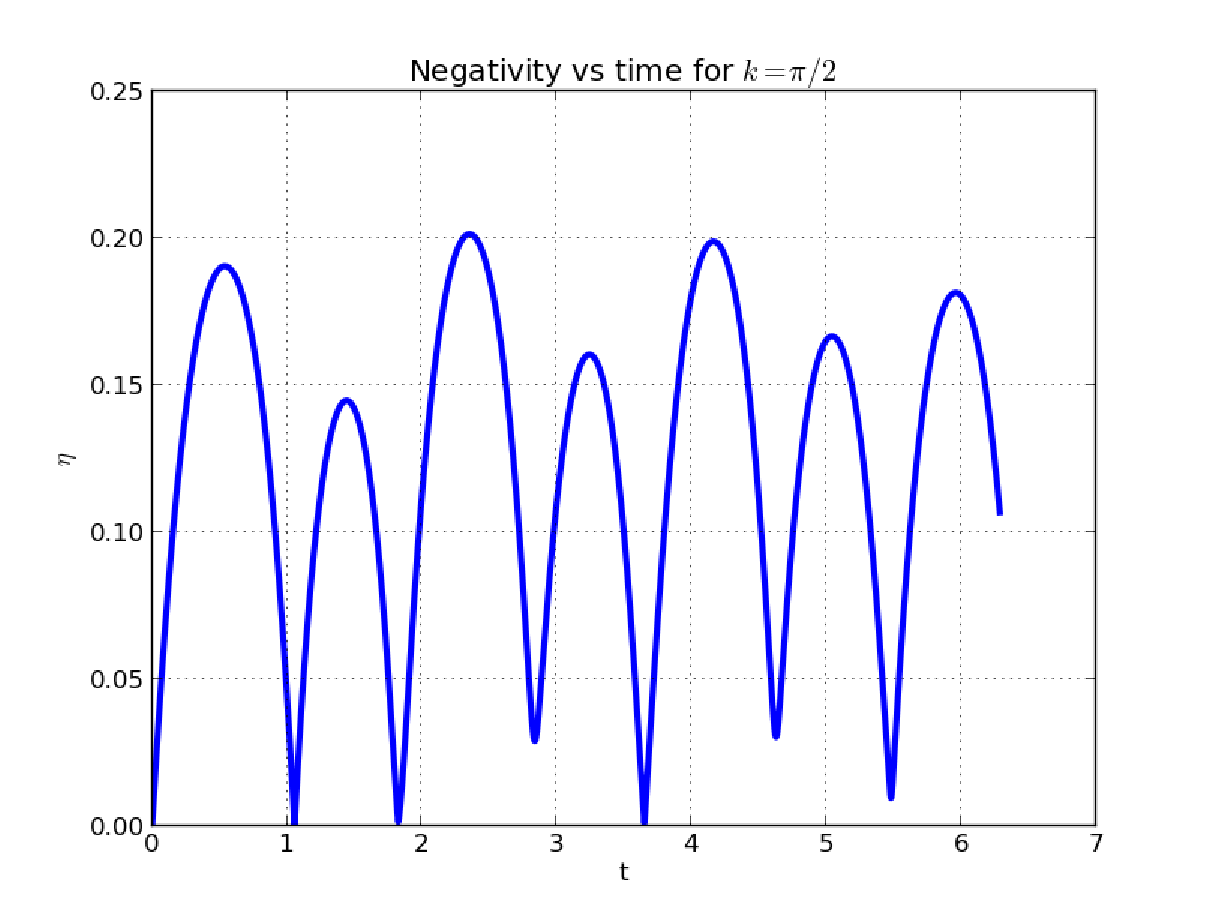
\includegraphics[scale=0.75]{figure1.pdf}
\caption{The negativity $\eta$ only depends on the elapsed time $t$ when the coupling constant $k_z$ is fixed.  This plot is for a fixed coupling coefficient of $k_z=\pi/2$ (and given the assumptions discussed in the text).}
 \label{fig:plot1}
\end{figure}
Fig.\ \ref{fig:IIplot2} is the behavior of the negativity as a function of the coupling coefficient if the time is fixed at $t=\pi/2$.  
\begin{figure}[th]
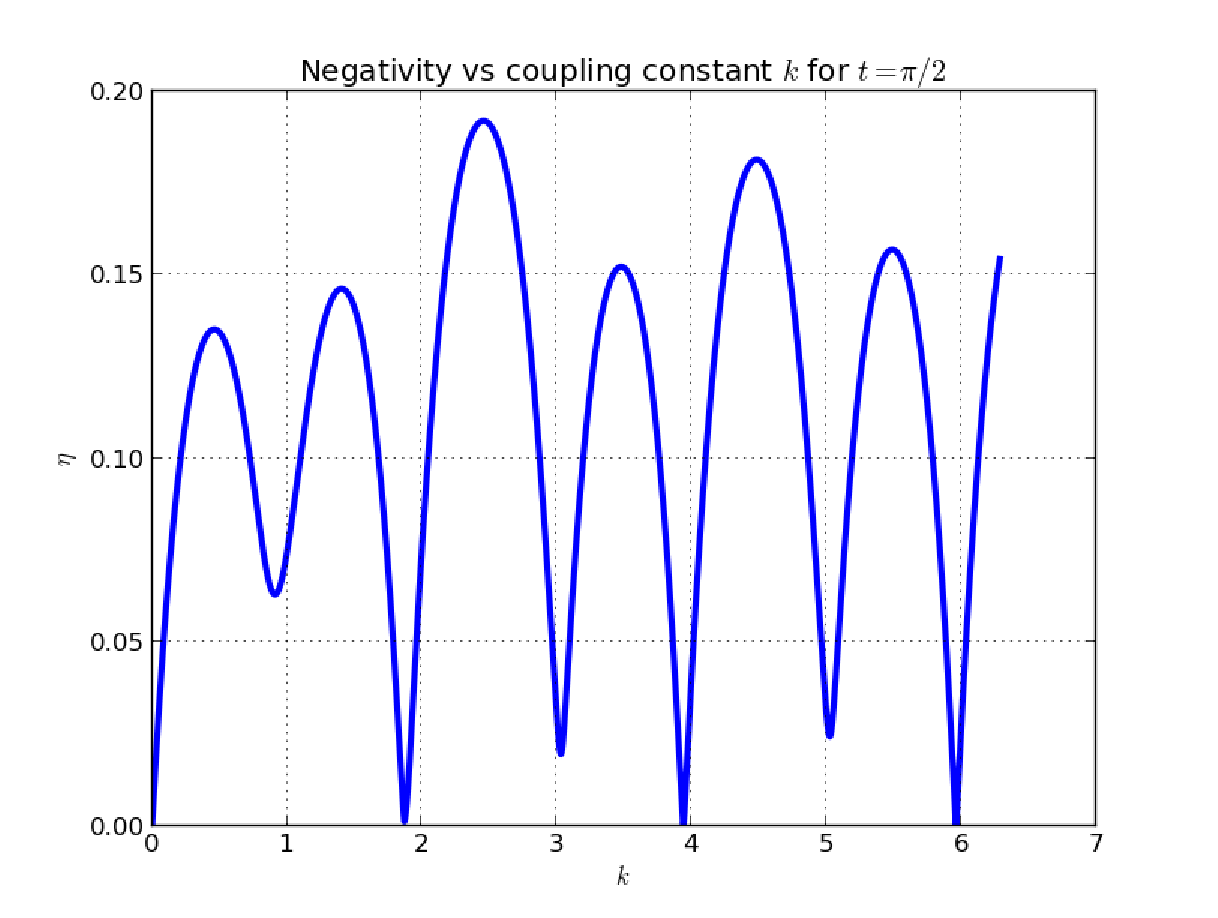
\includegraphics[scale=0.75]{figure2.pdf}
 \caption{The negativity $\eta$ only depends on  the coupling constant $k_z$ when the elapsed time $t$ is fixed.  This plot is for a fixed time of $t=\pi/2$.  (See the text for a discussion of the other assumptions.)}
\label{fig:IIplot2}
 \end{figure}
Both plots show the channel negativity $\eta$ calculated with one parameter (either $t$ or $k_z$) over the range $[0,2\pi]$ while holding the other parameter fixed.  Notice that the negativity is only zero (i.e.\ the channel is only completely positive) at a small number of fixed points.
 
The negativity can be plotted as a function of both the coupling coefficient and time for a visualization of the 2-dimensional parameter space over the range $[0,\pi]$.  Fig.\ \ref{fig:IIIplot3} is that plot.
\begin{figure}[th]
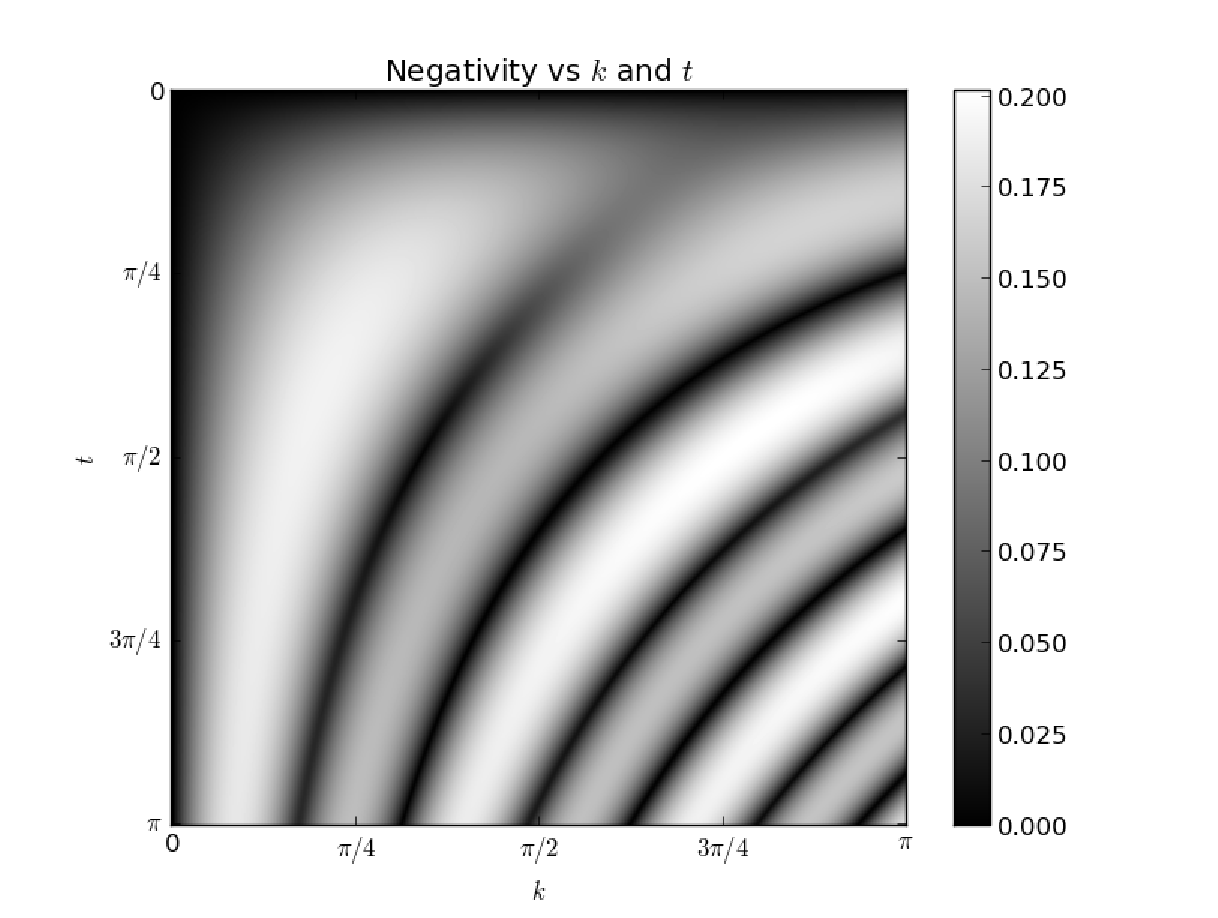
\includegraphics[scale=0.75]{figure3.pdf}
\caption{The negativity $\eta$ of the example Rabi channel in the text depends on both the coupling constant $k_z$ and the elapsed time $t$.  Notice that the channel is almost always negative, and the negativity appears cyclic.  The text discusses the assumptions used to produce this plot.}
 \label{fig:IIIplot3}
\end{figure}

This more complicated example shows that the negativity is dependent on the physical parameters of the Hamiltonian.  As such, a measurement of the negativity (through a tomography experiment) will yield information about parameters that might be inaccessible directly, e.g.\ the coupling $k_z$ between the reduced system and bath qubits in this Rabi channel.
 
The double Rabi atom universe presented here shows that theoretically negative channels can be found even with experimentally motivated Hamiltonians.  

Is it possible to create negative channels in the lab?  This question is of paramount importance.  The theoretical work presented so far seems to imply such a claim, but an experiment that measures the negativity of some channel in the lab (and compares it to the theoretical predictions presented here) is the only way to really answer this question.  Before exactly such an experiment is proposed, an important theoretical issue needs to be addressed:  Every channel presented so far has depended on the sharp operation $\vec{\tau}^\sharp=\vec{\tau}\otimes\left(R:\vec{\tau}:R^\dagger\right)$ where $R$ is some unitary rotation.  Is such a sharp operation physically reasonable?  Is it possible such a sharp operation might occur in nature?  Both of these questions will be answered in the next section.


\chapter{Physical Motivations for Sharp Operations}
\label{sec:sharp}

Sharp operations can be thought of as a by-product of the preparation procedure.  Every quantum experiment must begin with a preparation in some way at some point in time, and preparing the reduced system will only leave the bath completely unaffected if the reduced system is isolated.  In such cases, there is no need to discuss baths, complete positivity, or sharp operations.

Sharp operations of the form described here (i.e.\ linear and consistent, but not necessarily positive) have been discussed in \cite{Rodriguez2010} under the more typical name of assignment maps.  In that work, sharp operations of this form are proven to be Hermiticity- and trace-preserving.  In \cite{Sudarshen2007}, it is argued that the reduced dynamics described throughout this work should be thought of more as theoretical tools that are not necessarily compatible with the ``process map'' output of tomography experiments.  A process map is the superoperator found experimentally with a tomography experiment, and the reduced dynamics (which include the sharp operation) form a ``dynamical map'' that will have some positivity domain that may depend on the initial correlations of the reduced system and bath.  This is the key idea here.  In the language of \cite{Sudarshen2007}, a process map and a dynamical map both describe the same physical process only if the initial correlations are correctly accounted for in the sharp operation.  I. e.\ the theoretical description of such channels (``dynamical maps'') will coincide with experimental reality (``process maps'') only if the sharp operation accurately describes the initial correlation between the reduced system and the bath.  This concern is precisely why it is important to determine if the sharp operations we use can be created in the lab.   

It might be argued that the example sharp operation of 
\begin{equation}
\label{eqn:sharpref}
\tau_i = \tau_i\otimes \left(H_d\tau_i H_d^\dagger \right)\;\;,
\end{equation}
where $\tau_i$ is the $i$th states of the tomography vector $\vec{\tau}$ and $H_d$ is the Hadamard operator (Sec.\ \ref{sec:negexample} shows this sharp operation in use), does not have a simple physical interpretation.  To address such concerns, consider the situation arising when the reduced system and the bath are initially entangled in the state
$$
\ket{\Psi} = \frac{\ket{0+}+\ket{1-}}{\sqrt{2}}\;\;.
$$
Preparing the tomography states on the reduced systems yields
\begin{eqnarray*}
\ketbra{0}{0}\otimes I\ket{\Psi} &=& \ket{0+}\\
\ketbra{1}{1}\otimes I\ket{\Psi} &=& \ket{1-}\\
\ketbra{+}{+}\otimes I\ket{\Psi} &=& \ket{+0}\\
\ketbra{+_i}{+_i}\otimes I\ket{\Psi} &=& \ket{+_i}\left(\ket{+}-i\ket{-}\right),
\end{eqnarray*}
up to a normalization factor\footnote{The normalization term is left out of the expressions in this section for convenience and because it is not relevant to the argument.}.  These states do not exactly correspond to the sharp operation of Eqn.\ \ref{eqn:sharpref}.  Define a new sharp operation on $\vec{\tau}$ using the above projective measurements, i.e.\
\begin{equation}
\label{eqn:sharpPP}
\tau_i^{\sharp_p} = \frac{\left(\tau_i\otimes I\right) \ketbra{\Psi}{\Psi} \left(\tau_i\otimes I\right)}{\trace{\left(\left(\tau_i\otimes I\right)\ketbra{\Psi}{\Psi}\right)}}\;\;.
\end{equation}
Notice, $\tau_i^\sharp=\tau_i^{\sharp_p}$ for $i\in\{1,2,4\}$ but not for $i=3$.  However, $\left(Z_c\tau_{i}^\sharp Z_c^\dagger\right)^\flat = \left(Z_c\tau_{i}^{\sharp_p} Z_c^\dagger\right)^\flat\;\forall i$.  This observation makes it clear that the Choi matrix for a single qubit channel with composite dynamics described by $Z_c$ (i.e.\ Eqn.\ \ref{eqn:CZneg}) will be the same regardless of whether the sharp operation is described bb Eqn.\ \ref{eqn:sharpref} or Eqn.\ \ref{eqn:sharpPP}.

The above sharp operation can be explained as the reduced system and the bath initially being entangled in the pure state $\ket{\Psi}$ and then ideally preparing a tomography state on the reduced system.  The appearance of negative channels after projective measurements of reduced systems entangled with the bath is currently an active area of research \cite{Devi2011}.

A sharp operation does not always need to be explained with prior entanglement between the reduced system and the bath.  As pointed out in \cite{Sudarshen2007}, the two main preparation procedures in quantum mechanics are the ``preparation by measurement'' described above and ``stochastic preparations'' \cite{Sudarshen2007}.  Stochastic preparations are preparations of a system by setting some macroscopic parameter (e.g.\ the temperature or external magnetic field) and letting the system reach some equilibrium state.  For example, if the qubit is represented by the spin of an electron in a quantum dot, then preparation of only that spin by cooling would require the spatial extent of the cooling to be bounded by the spatial extent of the quantum dot.  This experimental requirement might not be met; the entire sample containing the quantum dot might be cooled resulting in every other spin in neighboring quantum dots to be similarly be prepared.  Every qubit would be prepared identically because every qubit is represented by a spin in the same (presumably spatially uniform) temperature field.  This situation is exactly described by the sharp operation
$$
\rho^\sharp = \rho\otimes\rho\otimes\rho\otimes\cdots\;\;.
$$
This situation is a simple example of a sharp operation which requires no prior entanglement between the reduced system and bath.

The conclusion is that sharp operations can be implemented in the lab as preparation procedures; as such, sharp operations are physical.  If quantum operations must be completely positive to be considered physically reasonable and if the controlled-phase gate and sharp operation of Eqn.\ \ref{eqn:sharpref} are both physically reasonable, then what part of the evolution described by Eqn.\ \ref{eqn:CZneg} is not physically reasonable?  The partial trace seems to be the only other major element of the mathematical description of that channel and the partial trace operation is well established in physics as a linear and positive operation \cite{Carlen2010} with a clear physical interpretation involving the consistency of expectation values in extended Hilbert spaces \cite{Cohen1992}.

Sharp operations represent preparation procedures in the open systems setting.  Negative channels can arise if the preparation procedure is not perfect or if the reduced system and bath are entangled prior to the preparation procedure.  Both situations can (and probably do) happen in nature.  It will be shown in later sections that a controlled ``bath'' will allow an experimenter to engineer a desired sharp operation and experimentally measure the negativity of a channel.  
 
\chapter{Negative Qubit Channel Examples With Multi-Qubit Baths}
\label{sec:multibath}

The example channel $(\vec{\tau},\vec{\tau}\otimes \left( H_d:\vec{\tau}:H_d^\dagger\right),D)$ can be extended by redefining the $4\times4$ matrix $D$ as an $2^M\times 2^M$ matrix $D^\prime$.  This new channel describes a qubit channel with a bath of $M-1$ qubits as opposed to the single qubit bath of all the previous examples.  The larger bath will also require a different sharp operation.  Suppose,
$$
\vec{\tau}^\sharp = \vec{\tau}\otimes\left(H_d:\vec{\tau}:H_d^\dagger\right)\otimes\bigotimes_{i=3}^{M}\ketbra{0}{0}\;\;;
$$
i.e.\ the first bath qubit will act exactly as the only bath qubit of the previous examples and the rest of the bath qubits will simply be prepared in a fixed state of $\ketbra{0}{0}$.  This sharp operation could arise, for example, from a combination of the stochastic and measurement preparation methods described in the previous section.  The entire system might be cooled to the ground state $\ketbra{0}{0}$ except for two qubits that somehow manage to remain maximally entangled.  Preparation of the reduced system in the ``preparation by measurement'' manner described in the previous section could then result in this sharp operation.  Notice,
$$
\varepsilon(\rho) \equiv \left(D^\prime \rho^\sharp D^{\prime\dagger}\right)^\flat = \begin{pmatrix}x&y\\y^*&1-x\end{pmatrix}
$$
where
$$
x = \sum_{i=1}^{2^{M-1}} \rho^\sharp_{ii}
$$
and
$$
y = \sum_{i=1}^{2^{M-1}} \sum_{j=(2^{M-1})+1}^{2^M} D^\prime_{i} \rho^\sharp_{ij} D^{\prime *}_j\;\;.
$$
The complex number $D^\prime_i$ is the $i$th diagonal element of $D^\prime$ and $\rho$ is some valid density matrix.  This is the straightforward extension of Eqn.\ \ref{eqn:exrd1} to a multi-qubit bath.  The transformation matrix $\hat{R}$ from that section can be used to find    
\begin{eqnarray*}
\varepsilon(\vec{\tau}) &=& \left(\begin{pmatrix}
1&0\\0&0
\end{pmatrix},\right.\\
& &\frac{1}{4}\begin{pmatrix}
0&D^\prime_s D^{\prime *}_1-D^\prime_{s+r}D^{\prime *}_{1+r}\\
3D^\prime_1 D^{\prime *}_s+D^\prime_{1+r}D^{\prime *}_{s+r}&0
\end{pmatrix},\\
& &\frac{1}{4}\begin{pmatrix}
0&3D^{\prime *}_1 D^{\prime}_s+D^{\prime *}_{1+r}D^{\prime}_{s+r} \\
D^{\prime *}_s D^{\prime}_1-D^{\prime *}_{s+r}D^{\prime}_{1+r}&0
\end{pmatrix},\\
& &\left.\begin{pmatrix}
0&0\\
0&1
\end{pmatrix}\right)\;\;,
\end{eqnarray*}
with $s=(2^{M-1})+1$ and $r=2^{M-2}$, which leads to a Choi representation of this channel of
\begin{equation}
\label{eqn:choiIII}
C_{D^\prime} = \mathbf{C}\odot\left(D^\prime :\vec{\tau}^\sharp : D^{\prime\dagger}\right)^\flat = \begin{pmatrix}
1&0&0&m\\
0&0&n&0\\
0&n^*&0&0\\
m^*&0&0&1
\end{pmatrix}
\end{equation}
with
$$
m = 3D^{\prime *}_1 D^{\prime}_s+D^{\prime *}_{1+r}D^{\prime}_{s+r}
$$
and
$$
n = D^{\prime *}_s D^{\prime}_1-D^{\prime *}_{s+r}D^{\prime}_{1+r}\;\;.
$$
The spectrum of this channel would be
$$
\operatorname{spec}\left(C_{D^\prime}\right)=\left(1-\sqrt{mm^*},1+\sqrt{mm^*},-\sqrt{nn^*},\sqrt{nn}\right)\;\;,
$$
with
$$
\pm \sqrt{mm^*} = \pm \frac{1}{\sqrt{8}}\sqrt{5+3\cos(f_\nu t)}
$$
and
$$
\pm \sqrt{nn^*} = \pm\frac{1}{2} \sin\left(\frac{f_\nu t}{2}\right)\;\;.
$$
The argument $f_\nu$ is defined in terms of the composite Hamiltonian that generates $D^\prime$, similar to Eqn.\ \ref{eqn:ftheta}; i.e.\
$$
f_\nu = \nu_1-\nu_{1+r}-\nu_s+\nu_{s+r}\;\;,
$$
where $\nu_i$ is the $i$th eigenvalue of the composite Hamiltonian.  Notice (with $\hbar=1$)
$$
f_\nu t = 2\pi n\Rightarrow \eta_{D^\prime} = 0
$$
where $n\in\mathbb{Z}$, $t$ is the elapsed time defining $D^\prime$ and $\eta_{D^\prime}$ is the negativity of this example $M$ qubit channel.  This channel is, like most of the previous examples, almost always negative.  The addition of a multi-qubit bath does not force complete positivity.  

In general,
\begin{equation}
\label{eqn:formref}
\rho^\sharp = \rho\otimes b = \begin{pmatrix} \rho_{11} b& \rho_{12} b\\ \rho_{21} b&\rho_{22} b\end{pmatrix}
\end{equation}
where $\rho\in\mathcal{S}(\mathcal{H}^S)$ is the reduced system state (a single qubit) and $b\in\mathcal{S}(\mathcal{H}^B)$ is some bath state (not necessarily a single qubit), and
\begin{eqnarray*}
D\rho^\sharp D^\dagger &=& D\left(\rho\otimes b\right)D^\dagger \\
&=& \begin{pmatrix} D_1 & 0 & \cdots & 0\\ 0 & \ddots & \ddots & \vdots \\ \vdots & \ddots & \ddots & 0 \\ 0 & \cdots & 0 & D_{2^M}\end{pmatrix} \begin{pmatrix} \rho_{11} b& \rho_{12} b\\ \rho_{21} b&\rho_{22} b\end{pmatrix}  \begin{pmatrix} D_1^* & 0 & \cdots & 0\\ 0 & \ddots & \ddots & \vdots \\ \vdots & \ddots & \ddots & 0 \\ 0 & \cdots & 0 & D_{2^M}^*\end{pmatrix}
\end{eqnarray*}
These equations imply
$$
x= \sum_{i=1}^{2^{M-1}} \rho^\sharp_{ii} = \rho_{11} \trace(b) = \rho_{11}
$$
and
$$
y = \sum_{i=1}^{2^{M-1}} \sum_{j=(2^{M-1})+1}^{2^M} D^\prime_{i} \rho^\sharp_{ij} D^{\prime *}_j = \sum_{i=1}^{2^{M-1}} \sum_{j=(2^{M-1})+1}^{2^M} \rho_{12} D^\prime_{i} b_{ii} D^{\prime *}_j = \kappa_b \rho_{12}\;\;,
$$
with $\kappa_b = \sum_{i=1}^{2^{M-1}} \sum_{j=(2^{M-1})+1}^{2^M} D^\prime_{i} b_{ii} D^{\prime *}_j$.  This implies the reduced dynamics on the canonical tomography basis can be written down as
$$
\varepsilon(\vec{\tau}) = \left(\begin{pmatrix}
1&0\\0&0
\end{pmatrix},\frac{1}{2}\begin{pmatrix}
1&\kappa_+\\\kappa_+^*&1
\end{pmatrix},\frac{1}{2}\begin{pmatrix}
1&-i\kappa_{+_i}\\i\kappa_{+_i}^*&1
\end{pmatrix},\begin{pmatrix}
0&0\\0&1
\end{pmatrix}\right)\;\;,
$$
where $\kappa_+$ is a function of the bath state $b_+$ resulting from the sharp operation acting on $\ketbra{+}{+}$ and $\kappa_{+_i}$ is a function of some other bath state $b_{+_i}$ resulting from the sharp operation acting on $\ketbra{+_i}{+_i}$.  The Choi representation of this channel is of the form of Eqn.\ \ref{eqn:choiIII} with
$$
m = \frac{\kappa_++\kappa_{+_i}}{2}
$$
and
$$
n = \frac{\kappa_+^*-\kappa_{+_i}^*}{2}\;\;.
$$
This channel will be negative when $nn^*\neq 0$.  

The evolution of a single qubit in a sea of qubits will, presumably, be a common problem in the world of quantum technologies.  The reduced system qubit is not required to be initially correlated with all of the bath qubits or even some fixed majority of them.  The qubit channel will almost always be negative if the reduced system qubit is initially correlated to a single member of the $M$ qubit bath.  

This problem becomes much more difficult when considering continuous baths, as is usually the case in the study of open quantum systems.  In general, the Liouville-von Neumann evolution of the composite system will always lead to reduced system dynamics independent of complete positivity assumptions; i.e.\
$$
\dot{\rho} = -\frac{i}{\hbar} \left([H^{SB},\rho^\sharp]\right)^\flat
$$
describes the reduced system dynamics where $H^{SB}\in\mathcal{B}(\mathcal{H}^{SB})$ is the composite Hamiltonian governing the composite dynamics and $\rho\in\mathcal{S}(\mathcal{H}^S)$ is the state of the reduced system.  This equation does not require any assumptions of complete positivity.  

Unfortunately, this equation is also unwieldy and resistant to analytical analysis.  As a result, several assumptions are typically used to derive simpler evolution equations.  The Markovian master equation, also called the ``Lindblad'' or ``Kossakowski-Lindblad'' equation, is an example of such a simplification, and it takes the form  
\begin{equation}
\label{eqn:lind}
\mathcal{L}\rho^S(t) = -i[H,\rho(t)] + \sum_{k=1}^{N^2-1} \gamma_k \left( A_k\rho^S(t) A_k^\dagger - \frac{1}{2}A_k^\dagger A_k\rho^S(t) - \frac{1}{2} \rho^S(t)A_k^\dagger A_k\right)\;\;,
\end{equation}
where $\gamma_k\ge 0\;\forall k$ and the operators $A_k$ are called ``Lindblad'' operators.  The operator $H$ will generate the unitary (i.e.\ Hamiltonian) dynamics of the evolution, but in general, $H$ is not equal to the system Hamiltonian, and in the literature, $H$ is usually referred to as the ``Hermitian part'' of the system Hamiltonian.  The derivation of this equation can be found in \cite{Breuer2007}.  The important points for this discussion are the assumptions that lead to this equation.

The first key assumption in the derivation of Eqn.\ \ref{eqn:lind} is the semigroup property.  Suppose the dynamics of the reduced system from times $t=0$ to $t$ are represented as
$$
\rho^S(t) = V(t)\rho^S(0)\;\;. 
$$
The map 
$$
V(t) : \mathcal{S}(\mathcal{H}^S) \rightarrow \mathcal{S}(\mathcal{H}^S)
$$
is called a ``dynamical map''.  The dynamical map $V(t)$ is defined for a fixed time $t\ge0$, and allowing $t$ to vary produces the one-parameter family $\{V(t)|t\ge0\}$ of dynamical maps which completely describe the future time evolution of the open system.  Here, it is assumed that memory effects of the bath are negligible; i.e.\ the evolution is Markovian.  This idea is made formal with the semigroup property
$$
V(t_1)V(t_2) = V(t_1+t_2),\;\;\;t_1,t_2\ge0\;\;.
$$

The introduction of this rule creates a semigroup from the one-parameter family $\{V(t)|t\ge0\}$ of dynamical maps.  The semigroup of dynamical maps has a multiplication operation among the group elements defined by the above Markov rule but each group element does not necessarily have an inverse, hence the collection of dynamical maps only forms a {\it semi}group.

Given a semigroup of dynamical maps, there must be some linear operator $\mathcal{L}$ that will allow the semigroups to be represented in exponential form as
$$
V(t) = e^{\mathcal{L}t}\;\;.
$$
This description of the dynamical map $V(t)$ in terms of some generator $\mathcal{L}$ might seem to come out of the blue, but it is in fact a well established property of dynamical semigroups.  The reference \cite{Engel1999} gives all the gory details, but a brief explanation can be seen as follows:  Remember the dynamical semigroup is defined by the semigroup property $V(t_1)V(t_2) = V(t_1+t_2)$ for $t_1,t_2\ge0$.  Above, $\rho(t) = V(t)\rho(0)$ was given as a definition of the map $V(t)$.  Hence $\rho(0)=V(0)\rho(0)$, or
$$
V(0) = I\;\;.
$$
This initial value and the semigroup property actually form the meat of a famous functional equation posed by Cauchy in 1821.  Cauchy wanted to find all maps $T(\cdot): \mathbb{R}_+\rightarrow \mathbb{C}$ that satisfy the functional equation
$$
T(t+s) = T(t)T(s)\;\;\forall\; t,s \ge 0\;\;,
$$
with
$$
T(0) = 1\;\;.
$$
The exponential functions solve this functional equation, i.e.
$$
T(t) = e^{t\alpha}
$$
for any $\alpha\in \mathbb{C}$.  It turns out that all solutions of this functional equation will have this form \cite{Engel1999}.  

Notice the definition $T(t) := e^{t\alpha}$ for some $\alpha \in \mathbb{C}$ and all $t\ge 0$ implies $T(\cdot)$ is differentiable and satisfies the differential equation
$$
\frac{ d }{dt} T(t) = \alpha T(t)\;\;,
$$
with the initial value $T(0) = 1$.  The converse is also true: the function $T(\cdot): \mathbb{R}_+\rightarrow \mathbb{C}$ defined by $T(t) = e^{t\alpha}$ for some $\alpha \in \mathbb{C}$ and all $t\ge 0$ are the only functions that satisfy the above differential equation.  The proof of this proposition and its converse can both be found in \cite{Engel1999}.  

The semigroup structure of dynamical maps comes about from basic physical assumptions, i.e.\ the assumption of Markovian evolutions and the ability to compose dynamical maps.  Any family of maps obeying the given functional equation can be rewritten in terms of a generator obeying a differential equation.  Hence, these quantum dynamical maps can be thought of in terms of a generator $\mathcal{L}$ (called the ``Liouvillian'').  Dealing with the generator rather than the maps themselves is the great power of quantum dynamical semigroup theory.  As Engel says \cite{Engel1999}:

``...in most cases a complete knowledge of the maps $T(\cdot)$ is hard, if not impossible, to obtain.  It was one of the great discoveries of mathematical physics, based on the invention of calculus, that, as a rule, it is much easier to understand the `infinitesimal changes' occurring at any given time.  In this case, the system can be described by a differential equation replacing the functional equation...''

The derivation of the generator $\mathcal{L}$ of the dynamical maps $V(\cdot)$ requires the same replacement of the functional equation by the appropriate differential equation.  The derivation leads to Eqn.\ \ref{eqn:lind} when a few other assumptions are made \cite{Breuer2007}.  For our purposes, the most important of these other assumptions is compete positivity.

In the derivation of Eqn.\ \ref{eqn:lind}, it is assumed that the dynamical maps $V(t)$ are completely positive; hence, by the representation theorem,
$$
V(t)\rho^S = \sum_{\alpha} W_{\alpha}(t)\rho^S W_{\alpha}^\dagger(t)
$$
with some (time dependent) Kraus operators $W_\alpha$.  Negative channels have an operator sum representation, so it is tempting to just define
$$
V(t)\rho^S = \sum_\alpha \lambda_\alpha W_\alpha^\prime(t) \rho^S W_\alpha^{\prime\dagger}(t)
$$
and derive a new Lindblad equation that depends on the (possibly negative) eigenvalues of the Choi representation $\lambda_\alpha$.  Such an argument would imply that the only difference between the standard Lindblad equation and a ``negative Lindblad equation'' are coefficients, but such an argument would be misguided.

The problem with negative channels is much deeper than negative signs in the operator sum.  The assumption of Markovian evolution, i.e.\
$$
V(t_1)V(t_2) = V(t_1+t_2),\;\;t_1,t_2\ge 0
$$ 
assumes composability of the dynamical maps $V(t)$.  Any two completely positive dynamical maps can be composed.  A completely positive dynamical map will have a positivity domain which includes every possible reduced system state.  This fact may also be true of a negative dynamical map, but it is not required.  Two negative dynamical maps might have different (perhaps even non-overlapping) positivity domains, and it is not clear how two such maps could be composed.  It might be assumed that the composition of two negative maps would simply result in a new negative map with a new restricted positivity domain that is a function of the positivity domains of the two original maps.  Notice, however, that it would need to be proven that this new restricted positivity domain is non-empty.  Many examples have already been given of negative channels with positivity domains that are not all of the reduced system space.  Given two channels, if the first is a constant channel that sends every input state to a state that is not in the positivity domain of the second channel, then the combined, restricted positivity domain of their composition must be empty.  This example points out a serious issue with defining composition over negative dynamical maps in a general way.  It is not clear that negative dynamical maps have any kind of semigroup structure or that they can, in general, be described in terms of a generator in the manner shown above.  It should be noted, however, that if the negative maps do form a continuous semigroup, then extending the above equations to include negative channels can be done straightforwardly \cite{Shaji2005}.

The composition of negative channels is an open question.  Without an answer to this question, more complicated questions about the mathematical structure of the set of all negative channels will not have very satisfactory answers.  Completely positive dynamical maps have nice mathematical features beyond the Kraus representation, not the least of which is their amenability to the powerful mathematical techniques of semigroup theory.  These features need to be better understood for negative channels, but until that understanding arrives, the Liouville-von Neumann equation is the best method for modeling negative channels with continuous baths.

\chapter{Proposed Experimental Demonstration of Negativity}
\label{sec:proposedexp}

One of the main ideas of the previous section is to illustrate {\em gedanken} experiments with non-zero negativity, and diagonal channels were used for the express purpose of creating examples that would be amenable to theoretical analysis.  Those experiments did not involve statistical errors or systematic errors due to experimental limitations.  The authors of \cite{Wood2009} provide a nice discussion of how statistical errors in a process tomography experiment might lead to non-zero negativities, but no such considerations were given to the gedanken experiments presented in the previous sections.  Hence, the negativity of those example channels cannot be a product of such experimental error.  

Channels implemented in the lab, however, will have experimental error.  There will be errors associated with preparing the reduced system (which would be manifested in the theory as errors in the sharp operation), implementing the reduced dynamics (which would be manifested in the theory as errors in the composite dynamics), and in implementing the tomography of the reduced system.  The theoretical channel
$$
\varepsilon(\vec{\tau})=\left(U:\vec{\tau}^{\;\sharp}:U^\dagger\right)^\flat\;\;,
$$
with $\{\vec{\tau}^\sharp\}_i\in\mathcal{S}(\mathcal{H}^{SB})$, $U\in\mathcal{B}(\mathcal{H}^{SB})$ and $\{\vec{\tau}\}_i\in\mathcal{S}(\mathcal{H}^{S})$ might be implemented in the lab as
$$
\varepsilon(\vec{\tau})^\prime = \left( U_\delta:\vec{\theta}^{\;\sharp}:U_\delta^\dagger\right)^\flat
$$
where $U_\delta$ is some non-perfect implementation of the composite dynamics and $\vec{\theta}$ might be very different from the desired $\vec{\tau}$.  

\begin{example}
For example, preparing the canonical tomography vector
$$
\vec{\tau}=\left(\ketbra{0}{0},\ketbra{+}{+},\ketbra{+_i}{+_i},\ketbra{1}{1}\right)
$$
is difficult in certain experimental situations and can only be done probabilistically.  The preparation of the state $\ketbra{0}{0}$ might be done in such a way that the reduced system is actually prepared in the mixed state
$$
\rho_0 = p \ketbra{0}{0} + (1-p) \frac{I}{2}
$$
with some $p\in[0,1]$.  This noisy preparation is actually of the form reported by \cite{Howard2006} in their process tomography experiments.  If every preparation resulted in a similar mixed state (i.e.\ the preparation of any of the tomography states leads to a $(1-p)$ probability of producing the completely mixed state), then
$$
\vec{\theta} = \left(\rho_0,\rho_+,\rho_{+_i},\rho_1\right)\;\;.
$$
Suppose the bath is (again) a single qubit and the sharp operation is the familiar
$$
\vec{\tau}^\sharp = \vec{\tau}\otimes \left(H_d:\vec{\tau}:H_d^\dagger\right)\;\;.
$$
The sharp operation is only defined on the tomography set, so the imperfect preparation state needs to be rewritten as
$$
\rho_j = p\ketbra{j}{j} + \frac{(1-p)}{2}I
$$
where $I$ is formed from the elements of the tomography set as $I=\ketbra{j}{j}+\ketbra{k}{k}$ and with $j=\{0,+,+_i,1\}$ and $k$ defined such that $\braket{k}{j}=0$.  The sharp operation applied to the above noisy state yields
\begin{eqnarray*}
\rho_j^\sharp &=& p\left(\ketbra{j}{j}\otimes H_d\ketbra{j}{j}H_d^\dagger\right) + \frac{(1-p)}{2}\left(\ketbra{j}{j}\otimes H_d\ketbra{j}{j}H_d^\dagger\right)+\frac{(1-p)}{2}\left(\ketbra{k}{k}^\sharp\right)\\
&=&\frac{(p+1)}{2}\left(\ketbra{j}{j}\otimes H_d\ketbra{j}{j}H_d^\dagger\right)+\frac{(1-p)}{2}\left(\ketbra{k}{k}^\sharp\right)\;\;.
\end{eqnarray*}
From the above equation it is clear that, unless $p=1$,
$$
\vec{\theta}^{\;\sharp} \neq \vec{\tau}^{\;\sharp}
$$
which implies
$$
U\rho_j^\sharp U^\dagger \neq U\ketbra{j}{j}^\sharp U^\dagger\;\;,
$$
and the imperfectly prepared channel will be different from the desired channel (as expected).   
\end{example}

The application of the sharp operation becomes suspect when considering ``noisy'' experiments.  Originally, the sharp operation was introduced as a map that correctly accounts for the initial correlation of the reduced system and bath on the states actually created in the lab.  The experimenter in the above example is not even sure what states are actually created in the lab.  The completely mixed state might not be in the positivity domain of the sharp operation used in the channel definition.  The sharp operation is, however, the experimenter's best guess for the initial correlation of the state he wants to create in the lab.  As such, the experimenter must assume he can create states close to the states he uses to define his sharp operation (e.g.\ in the above example, the experimenter must assume $p \approx 1$).  The theoretical predictions of the channel might not be testable (i.e.\ might not yield valid density matrices) without such an assumptions.  It can be assumed, however, if it was the case that $p<< 1$ in the above experiment, then the experimenter would declare his preparation procedure is be too flawed to actually conduct the tomography experiment.  These issues are all part of the difficulty in comparing the theoretical predictions of the mathematical representations of channels to their physical counterparts, and such issues are precisely why many authors stress the importance of remembering the difference between measured experimental data and predicted experimental data given a specific model (e.g.\ \cite{Sudarshen2007}).  For this discussion, it suffices to recognize that even if the sharp operation correctly describes the initial composite state correlation for the states the experimenter wishes to prepare, it might not do so for the states he actuals prepares, and the experimentally measured negativity might not match the predicted negativity in such a situation.

The imperfect preparation presented above is just a simple example of possible experimental error.  Many other situations can lead to similar results, i.e.\ an implemented channel which does not follow theoretical predictions.  Given these kinds of experimental errors, it can be expected that there will be differences in the negativity of the desired (i.e.\ theoretical) channel and the channel implemented in the lab.  It is important to be able to tell the difference between theoretically predicted negativity and experimental error negativity.  

Empirical evidence is required to confirm the theoretically predicted negativity, but experimental error cannot be predicted in detail (to eliminate its effects in the data post processing stage of the experiment) nor completely eliminated experimentally.  Realistic preparation and measurement procedures will contain errors, and tomographic characterization of a channel will involve statistical errors associated with the data collection and processing.  The correct form of the sharp operation and composite dynamics will involve educated guesswork about the bath and its interaction with the reduced system.  All of these issues will make it very difficult to theoretically predict the negativity that might be measured in the lab.  One possible solution is to perform experiments with a ``controlled bath''.

Every experiment will have a bath as defined in the introduction, but confirmation of theoretically predicted negativity will require creating an artificial bath under the control of the experimenter.  Controlling the bath allows the experimenter to engineer the sharp operation and composite dynamics to verify the theoretically predicted negativity within some predefined statistical confidence.  The experimenter will measure
$$
\eta_{\mathrm{measured}} = \eta_{\mathrm{theoretical}} + \eta_{\mathrm{error}}
$$
where $\eta_{\mathrm{error}}$ is some error term due to experimental errors that can (hopefully) be made small enough to confirm
$$
\eta_{\mathrm{measured}} = \eta_{\mathrm{theoretical}} \pm \Delta\;\;,
$$
where $\Delta$ is some ``acceptable error level''.  

The proposals below are for experiments with just such ``controlled baths'' that can be implemented in modern quantum optics labs.  

\section{Photonic Root-Swap Operation}

Quantum computing (or ``quantum information processing'') involves the application of a desired unitary operation to a specifically prepared initial state to achieve an output state that represents a solution to some computational problem.  The desired unitary operation can be represented in terms of individual single or multiple qubit operations called ``gates''.  Many gates are important in the quantum computing community, including the controlled NOT ($CX$) and the Toffoli gate, and are well studied both theoretically and experimentally.  Another such gate is the two qubit ``root-swap'' (or $\sqrt{Sw}$) gate which is applied twice to swap the state of two qubits.  The root swap gate is important to us because it leads to a negative channel for one of the input qubits.

The root swap gate is defined as
$$
U_{\sqrt{Sw}} = \frac{1}{\sqrt{2}}\begin{pmatrix}
\sqrt{2}&0&0&0\\
0&1&i&0\\
0&i&1&0\\
0&0&0&\sqrt{2}
\end{pmatrix}\;\;.
$$
One of the input qubits will be labeled the ``reduced system'' and the other will be the ``bath''.  The sharp operation relating the initial states of these two qubits will be the familiar 
$$
\vec{\tau}^\sharp = \vec{\tau}\otimes\left(H_d:\vec{\tau}:H_d^\dagger\right)\;\;,
$$
where $\vec{\tau}$ is the canonical tomography vector and $H_d$ is the Hadamard gate.  The output of the channel $(\vec{\tau},\sharp,U_{\sqrt{Sw}})$ will be found in the usual manner, i.e.\
$$
\varepsilon(\vec{\tau}) = \left(U_{\sqrt{Sw}}:\vec{\tau}^\sharp:U_{\sqrt{Sw}}^\dagger\right)^\flat
$$
which leads to the following Choi representation of the channel:
$$
C_{\sqrt{Sw}} = \mathbf{C}\odot\varepsilon\left(\vec{\tau}\right) =
\begin{pmatrix}
 \frac{3}{4} & -\frac{i}{2 \sqrt{2}} & \frac{1}{4} & \frac{\frac{1}{2}+\frac{i}{2}}{\sqrt{2}} \\
 \frac{i}{2 \sqrt{2}} & \frac{1}{4} & \frac{\frac{1}{2}-\frac{i}{2}}{\sqrt{2}} & -\frac{1}{4} \\
 \frac{1}{4} & \frac{\frac{1}{2}+\frac{i}{2}}{\sqrt{2}} & \frac{1}{4} & -\frac{i}{2 \sqrt{2}} \\
 \frac{\frac{1}{2}-\frac{i}{2}}{\sqrt{2}} & -\frac{1}{4} & \frac{i}{2 \sqrt{2}} & \frac{3}{4}
\end{pmatrix}\;\;.
$$
Notice
\begin{eqnarray*}
\operatorname{spec}(C_{\sqrt{Sw}}) &=& \left(\frac{1}{2} \left(1+\sqrt{2+\sqrt{2}}\right),\frac{1}{2} \left(1+\sqrt{2-\sqrt{2}}\right),\right.\\
& &\left. \frac{1}{2} \left(1-\sqrt{2+\sqrt{2}}\right),\frac{1}{2} \left(1-\sqrt{2-\sqrt{2}}\right)\right)
\end{eqnarray*}
and, more importantly,
$$
\eta_{\sqrt{Sw}} \approx 0.149\;\;.
$$

The root-swap gate has been accomplished on polarization state photonic qubits with a fidelity of about 90\% \cite{Cernoch2008}, and those experiments may be able to be modified to experimentally test negativity calculations.  

Figure \ref{fig:opticalneg} shows the optical set-up used by Cernoch et al.\ \cite{Cernoch2008}.  
\begin{figure}[h!t]
\centering
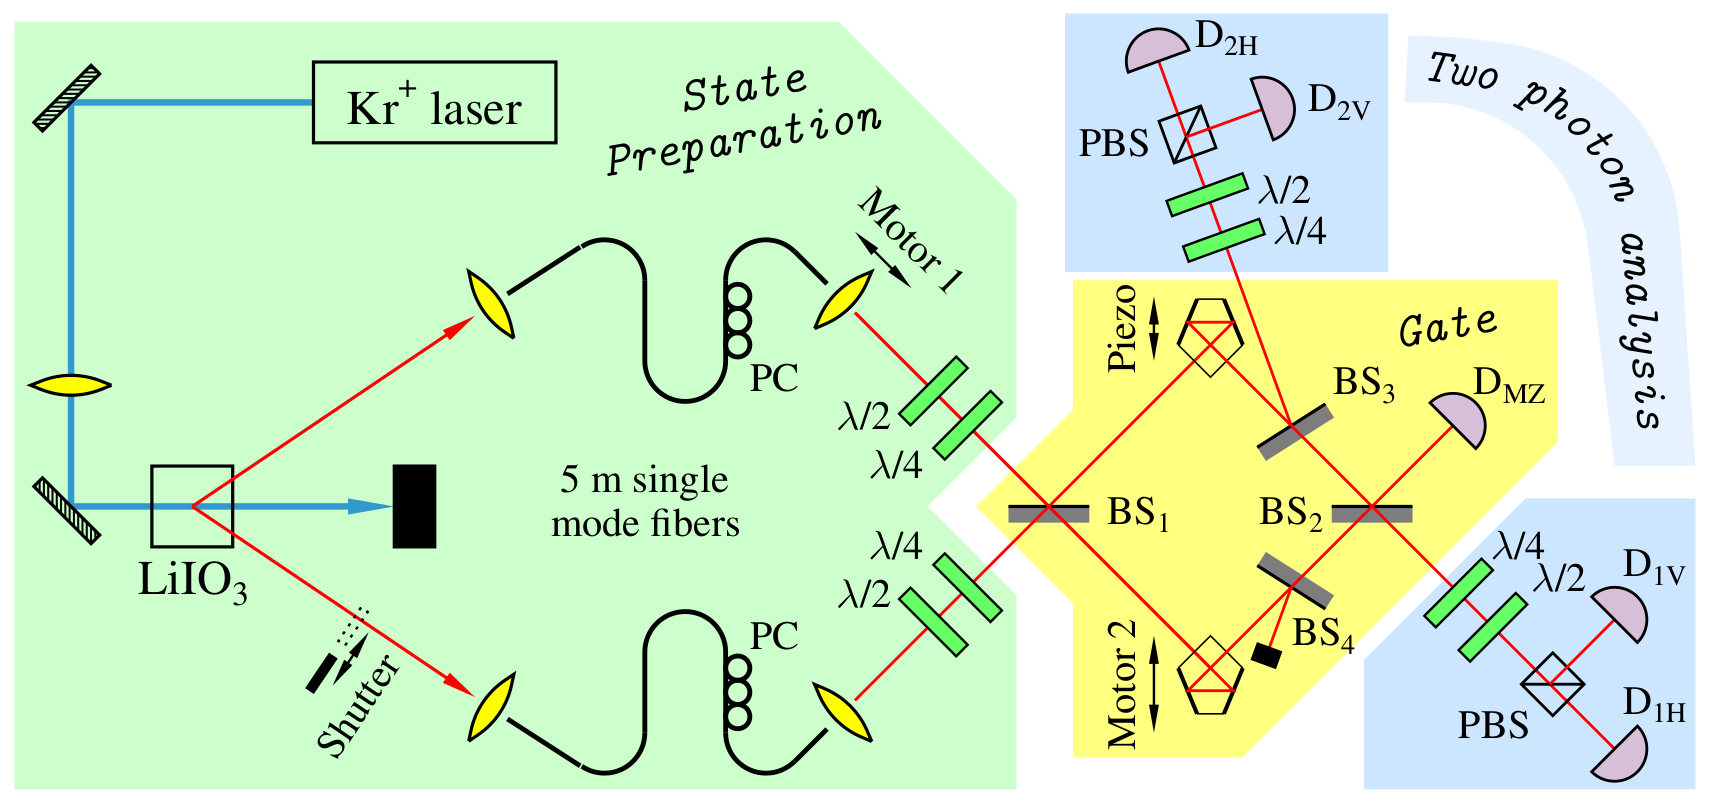
\includegraphics[scale=1.5]{opticalneg1.png}
\caption{This is the optical set-up used in \cite{Cernoch2008} to implement a root swap gate.  This experiment can be conducted in a slightly different manner to verify the theoretically predicted negativity of 0.149 for the channel induced by this gate on one of the two input qubits.  This diagram is reproduced with permission from \cite{Cernoch2008}.}
\label{fig:opticalneg}
\end{figure}
The yellow box in Fig.\ref{fig:opticalneg} (labeled ``Gate'') is the part of the process which implements the gate being investigated.  The gate implementation involves the Hong-Ou-Mandel effect and arbitrary phase shifts accomplished by using the motorized prisms to change the path lengths.  This optical set-up can be used to accomplish many different two qubit gates, but our interest is in the implementation of the root-swap gate.  See \cite{Cernoch2008} for all the details of this set-up, along with references to similar optical set-ups used to perform other gates.   

The authors of the above experiment performed process tomography to demonstrate that the action of the optical set-up in Fig.\ \ref{fig:opticalneg} can be made very close to the desired root swap\footnote{The experiment was far more than just the quantum process tomography.  It also involved fidelity and entanglement measurements, but those results do not concern the discussion here.}.  In principle, the raw data collected by this group was the superoperator representation of the two qubit channel implemented by Fig.\ \ref{fig:opticalneg}; i.e.\
$$
\mathbf{S} \odot \left( U_{\sqrt{sw}}^\prime: \vec{\xi} :U_{\sqrt{sw}}^{\prime\dagger}\right)
$$
where $U_{\sqrt{sw}}^\prime$ is the operation actually performed by the optical set-up in Fig.\ \ref{fig:opticalneg} and $\vec{\xi}$ is some two qubit tomography vector.  A maximum likelihood method was used on the raw data to find the ``reconstructed completely positive map''.

Notice that the experiment would need to be modified to calculate the negativity.  The negative channel is a single qubit channel.  The sharp operation on the single qubit tomography vector involves a Hadamard rotation on one of the qubits, and such a rotation was not present in the original experiment. 

If such modifications to the experiment can be made, then the desired single qubit channel can be measured.  For example, the LiIO$_3$ crystal in Fig.\ \ref{fig:opticalneg} is a type I source, which indicates that the output entangled pair could be written down as \cite{Kok2010}
$$
\frac{\ket{00}+\ket{11}}{\sqrt{2}}\;\;,
$$  
and the addition of a $\pi/4$ waveplate\footnote{This is a process that implements the Hadamard rotation in the sharp operation.  This could be accomplished, for example, with a half-wave plate oriented at 22.5 degrees from the optical axis \cite{Ralph2010}.} in one of the state preparation arms would lead to
$$
\left(I\otimes H_d\right) \frac{\ket{00}+\ket{11}}{\sqrt{2}} = \frac{\ket{0+}+\ket{1-}}{\sqrt{2}}\;\;.
$$  
The qubit in the arm without the $\pi/4$ waveplate would then be prepared with a projective measurement (e.g.\ with a polarization filter).  This new preparation procedure would implement the desired sharp operation, although it might significantly change the behavior of the gate.

Performing {\em single} qubit process tomography on one of the two qubits in this new experiment (i.e.\ with the correctly implemented sharp operation and root-swap gate) would lead to a superoperator (or Choi) representation from which the negativity could be measured.  In the introduction, one photon was labeled the ``reduced system'' and the other the ``bath'', but the distinction only matters in the value of the negativity, not in whether or not the negativity is non-zero.  This feature is important to the experimentalist who might have trouble identifying the photons in his experimental set-up.  To see this idea notice,
$$
\mathbf{C}\odot\left(U_{\sqrt{Sw}}:\vec{\tau}^\sharp:U_{\sqrt{Sw}}^\dagger\right)^\flat =
\begin{pmatrix}
 \frac{3}{4} & -\frac{i}{2 \sqrt{2}} & \frac{1}{4} & \frac{\frac{1}{2}+\frac{i}{2}}{\sqrt{2}} \\
 \frac{i}{2 \sqrt{2}} & \frac{1}{4} & \frac{\frac{1}{2}-\frac{i}{2}}{\sqrt{2}} & -\frac{1}{4} \\
 \frac{1}{4} & \frac{\frac{1}{2}+\frac{i}{2}}{\sqrt{2}} & \frac{1}{4} & -\frac{i}{2 \sqrt{2}} \\
 \frac{\frac{1}{2}-\frac{i}{2}}{\sqrt{2}} & -\frac{1}{4} & \frac{i}{2 \sqrt{2}} & \frac{3}{4}
\end{pmatrix}\Rightarrow \eta_{\sqrt{Sw}} \approx 0.149
$$
and
$$
\mathbf{C}\odot\trace_S\left(U_{\sqrt{Sw}}:\vec{\tau}^\sharp:U_{\sqrt{Sw}}^\dagger\right) =
\begin{pmatrix}
 \frac{3}{4} & \frac{1}{2 \sqrt{2}} & \frac{1}{4} & -\frac{\frac{1}{2}+\frac{i}{2}}{\sqrt{2}} \\
 \frac{1}{2 \sqrt{2}} & \frac{1}{4} & \frac{\frac{1}{2}+\frac{i}{2}}{\sqrt{2}} & -\frac{1}{4} \\
 \frac{1}{4} & \frac{\frac{1}{2}-\frac{i}{2}}{\sqrt{2}} & \frac{1}{4} & -\frac{1}{2 \sqrt{2}} \\
 -\frac{\frac{1}{2}-\frac{i}{2}}{\sqrt{2}} & -\frac{1}{4} & -\frac{1}{2 \sqrt{2}} & \frac{3}{4}
\end{pmatrix}\Rightarrow \eta_{\sqrt{Sw}} \approx 0.126\;\;.
$$
Tracing out either the ``bath'' or ``reduced system'' qubit in this experiment will lead to a negative channel.  The negativity can be experimentally determined as some value $\eta_{\sqrt{Sw}}^\prime$, and it is expected that
$$
\eta_{\sqrt{Sw}}^\prime = \eta_{\sqrt{Sw}} \pm \epsilon
$$
where $\epsilon$ is some small error term due to experimental (and statistical) error.  As stated before, such error is expected and cannot be eliminated completely.  Error in measurement is a part of experimental physics \cite{Taylor1997}.  Notice, however, unless $\epsilon\sim 10^{-1}$, the negativity found in the experiment should be greater than zero independent of which qubit is traced out.  

Further confirmation of the negative channel can be found by comparing the experimentally determined superoperator representation to the theoretically expected superoperator representation.  For example, a diamond norm\footnote{The diamond norm is a popular norm for comparing quantum operations.  It has ``a natural operational interpretation: it measures how well one can distinguish between two transformations by applying them to a state of arbitrarily large dimension'' \cite{Aroya2009} and was originally introduced in \cite{Kitaev1998}.} distance can be found between the two superoperators as
$$
\delta = ||S_m - S_t||_\diamond 
$$
where $S_t$ is the superoperator representation determined by the tomography data and 
$$
S_m = \mathbf{S}\odot\left(U_{\sqrt{Sw}}:\vec{\tau}^\sharp:U_{\sqrt{Sw}}^\dagger\right)^\flat
$$
or
$$
S_m = \mathbf{S}\odot\trace_S\left(U_{\sqrt{Sw}}:\vec{\tau}^\sharp:U_{\sqrt{Sw}}^\dagger\right)\;\;.
$$
If $\delta$ is sufficiently small (in the same way that $\epsilon$ above needs to be sufficiently small), then the measured superoperator representation $S_t$ would be said to be the expected representation of the desired single qubit channel.  

This proposed experiment is (theoretically) a straightforward extension of the Cernoch et al.\ \cite{Cernoch2008} experiment.  The experimental difficulties in implementing the suggested changes may be difficult, but they may not be insurmountable.

\section{Photonic CZ Operation}
\label{sec:CZprop}

The root swap gate is not the only two qubit gate that can be used to demonstrate a negative single qubit channel.  Another well studied gate is the controlled phase ($CZ$) gate which is defined as
$$
CZ = \begin{pmatrix}
1&0&0&0\\
0&1&0&0\\
0&0&1&0\\
0&0&0&-1
\end{pmatrix}\;\;.
$$
If one of the qubits is labeled the ``reduced system'' and the other the ``bath'', then the familiar sharp operation on the canonical tomography vector, i.e.\
$$
\vec{\tau}^\sharp = \vec{\tau} \otimes \left(H_d:\vec{\tau}:H_d\right)\;\;,
$$
will lead to reduced dynamics of
$$
\varepsilon(\vec{\tau}) = \left(CZ:\vec{\tau}^\sharp:CZ^\dagger\right)^\flat\;\;.
$$
The labeling will, just as in the previous subsection, be unimportant to the main idea (i.e.\ demonstrating a negative channel) because the negativity of the single qubit channel will be non-zero independently of which qubit is traced out of the experiment.  Notice,
\begin{equation}
\label{eqn:CZneg}
\mathbf{C}\odot \left(CZ:\vec{\tau}^\sharp:CZ^\dagger\right)^\flat = \begin{pmatrix}
 1 & 0 & 0 & \frac{1}{2} \\
 0 & 0 & \frac{1}{2} & 0 \\
 0 & \frac{1}{2} & 0 & 0 \\
 \frac{1}{2} & 0 & 0 & 1
\end{pmatrix}\Rightarrow\eta_{CZ} \approx 0.167 
\end{equation}
and
$$
\mathbf{C}\odot \trace_S\left(CZ:\vec{\tau}^\sharp:CZ^\dagger\right) = \begin{pmatrix}
 \frac{1}{2} & \frac{1}{2} & \frac{1}{2} & -\frac{1}{2}-\frac{i}{2} \\
 \frac{1}{2} & \frac{1}{2} & -\frac{1}{2}-\frac{i}{2} & -\frac{1}{2} \\
 \frac{1}{2} & -\frac{1}{2}+\frac{i}{2} & \frac{1}{2} & \frac{1}{2} \\
 -\frac{1}{2}+\frac{i}{2} & -\frac{1}{2} & \frac{1}{2} & \frac{1}{2}
\end{pmatrix}\Rightarrow\eta_{CZ} \approx 0.232\;\;.
$$
These expected negativities are on the same order as those of the previous subsection.

Many different proposals exist for implementing a $CZ$ gate with an optical set-up.  A good overview can be found in \cite{Kieling2012}.  Hofmann and Takeuchi suggest a way to implement a $CZ$ gate using only beam splitters and postselection \cite{Hofmann2002}, and Kiesel et al.\ have an another (but similarly simple) design for a $CZ$ gate using polarization dependent beamsplitters \cite{Kiesel2005}.  The main idea is that implementations of this gate in optical set-ups are well studied.  Any of these implementations may be capable of demonstrating the proposed negative channel.  

The complete experiment would involve the preparation of the tomography vector and sharp operation, and then the application of one of the above implementations of the $CZ$ gate.  The desired sharp operation is straightforward to implement in an optical set-up and can be done in exactly the same manner as described in the previous subsection: a non-linear crystal can be used to create an entangled pair of qubits, one of which is passed through a $\pi/4$ waveplate, the other of which is prepared with polarization filters.  The choice of encoding the qubit in the polarization of the photons means all of the desired operations can be accomplished with well understood polarization optics.  Most of the proposals for implementing the $CZ$ gate discussed above also use the polarization state of a photon as the qubit. 

These experiments provide exactly the desired ``controlled bath'' situation needed to experimentally study and verify the theoretical predictions of negativity.  The sharp operation can be changed by interchanging the $\pi/4$ waveplate in the preparation stage of the set-up with some other waveplate or with something more complicated like an EOM\footnote{An electo-optic modulater (EOM) is a crystal placed in an electric field that can be used to modulate the polarization of incoming photons.  The polarization of outgoing photons is related to the electric field strength applied to the crystal.}.  In this way, the theoretical predications concerning the impact of the sharp operation can be tested experimentally.  

The next logical step in understanding negative channels would be comparing the quantum process tomography data (without any kind of complete positivity forcing post processing) to simple models of more realistic baths.  The theoretical task in this process would be quite difficult because the sharp operations could only be assumed (or randomly guessed).  Negative channels should still be expected in these more ``realistic'' experiments (i.e.\ experiments without controlled baths), but the theoretical analysis of these experiment suffers the same problem that any open system analysis would suffer: finding the proper form for the bath.  Of course, such theoretical difficulties are irrelevant to the data collection process, and it can safely be assumed that experimental process tomography of negative channels has already happened in the literature.  This topic is explored further in the next section.

\chapter{Implications of Negative Channels}

The negativity of complicated experiments without controlled baths can be measured, and if the negativity were found to be non-zero in experiments predicted to have non-zero negativity, then the evidence for negative channels would be convincing, even if the exact negativity of such complicated experiments could not be predicted.  Such complicated experiments are actually common in the quantum information community and negative channels have probably already been observed (and promptly ``corrected'' in most cases).

Acceptance of the idea of negative channels might not change the field of quantum information in a fundamental sense; e.g.\ fundamental results such as no cloning and no signaling will still hold in general.  But, several small changes will need to be made in current experimental methods and some theoretical ideas will need to be changed to incorporate negativity.  This section aims to highlight a few examples of such changes and is a brief outline of some open questions about negative channels.

\section{Existing Experimental Evidence of Negative Channels}
\label{sec:Havel}

Environmental noise is considered a major obstacle to NMR systems as viable quantum information processing technologies \cite{Boulant2004}.  Such strong ties between the reduced system and the bath\footnote{For most NMR systems, the reduced system would be the individual nuclear spins addressed during the experiment and the bath would be the spin bath created by all the background spins of the material.} might be expected to lead to negative channels.

Consider an experiment conducted by Cory et al.\ \cite{Cory2004}, in which process tomography is performed on a three-qubit NMR quantum information processor.  The process being investigated is the quantum Fourier transform.  The process tomography of this experiment leads to a ``non-completely positive superoperator'', i.e.\ a negative channel.  

The authors state that the ``the spatial inhomogeneity in the RF (radio-frequency) field over the sample volume'' \cite{Cory2004} is the major contributing factoring to the observed negativity.  They go on to say that the superoperator measured under such conditions ``cannot be expected to precisely correspond to any physical process'' \cite{Cory2004}; i.e.\ it cannot be expected to be completely positive.    

Post-processing of the data is a way to guess what the ``correct'' (i.e.\ completely positive) process tomography data would be if the experimenters could implement the experiment without error.  To this end, the authors employ a ``CP-filtering'' technique \cite{Havel2003} and a ``positivity'' $\varrho$.  The positivity can be shown to be related to the negativity by the expression 
$$
\eta = \frac{1 - \varrho}{2 - \varrho}\;\;.
$$

The ``CP-filtering technique'' used by the authors forces the positivity to be 1, and it is clear that such a post processing method will always lead to a channel with zero negativity.  The authors take $\varrho=1$ as their condition for completely positivity in the same manner that $\eta=0$ if and only if the the channel is completely positive, and the ``CP filtering technique'' used in the post processing of the experimental data guarantees this result.

The positivity of the experimental data in this NMR experiment was $\varrho=0.60$, which corresponds to a negativity of $\eta\approx 0.29$.  This negativity was unexpected by the authors, but they note ```$\ldots$even though imposing the complete positivity constraint on the experimental observations did not change the supermatrix very much, the change was distinctly in the right direction since it improved the correlation with both the simulated and theoretical supermatrices.''  The ``CP-filtering technique'' is justified by better agreement of the ``filtered'' experimental data and the numerical simulations than between the raw experimental data and the numerical simulations.  

The authors probably very much desired a preparation procedure that would be represented by a sharp operation of the form $\rho^S\otimes\tau^B$ where $\rho^S$ is the desired state of the reduced system and $\tau^B$ is some fixed state of the bath.  This sharp operation would always lead to completely positive dynamics, and in that sense, the negativity is a mistake in the implementation of the desired preparation procedure.  

The point of this subsection is to illustrate an impact of accepting negative channels as physically reasonable (i.e.\ not ``mistakes'').  An experiment similar to the one in \cite{Cory2004} could be performed with numerical simulations which predict the observed negativities.  Such experiments would provide deeper insight not only into the experimental preparation procedure (and perhaps how to fix them) but also into the relationship between the reduced system and the bath.  

This paper \cite{Cory2004} is clear, in depth, and thorough.  It is also an example of something that is pervasive in process tomography experiments: post processing of experimental data to force complete positivity.  

\section{Restrictions Implied by Complete Positivity}

An a priori requirement of a vanishing negativity puts strong restrictions on theoretical models of quantum dynamics.  Perhaps most famously, Sudarshan \cite{Sudarshan1976} showed that complete positivity implies 
\begin{equation}
\label{eqn:T1}
T_1 \ge \frac{1}{2} T_2\;\;,
\end{equation}
where $T_1$ is the relaxation time for the magnetic polarization in the $z$ direction and $T_2$ is the relaxation time for the magnetic polarization in the $x$ and $y$ directions \cite{Sudarshan1978,Slichter1996,Bloch1946}.  $T_1$ is referred to as the ``population'' or ``occupation'' relaxation time, and $T_2$ is called the ``phase'' relaxation time.  These terms have found application throughout the field of quantum information, but they originated in the study of nuclear magnetization in the presence of external magnetic fields.  This result was derived directly from the Lindblad equation in \cite{Sudarshan1978}, but it can de derived from Redfield theory \cite{Slichter1996} or from other common open system approximations \cite{Skinner1987} \cite{Skinner1991}.  All such derivations assume complete positivity.  

The relaxation times of qubits are extremely important to understand.  Qubits must have the longest possible relaxations times for useful quantum information processing, and unjustified assumptions such as Eqn.\ \ref{eqn:T1} can hamper the field's attempts at engineering such devices.  The relationship between the occupation and phase relaxation times can be reconsidered using negative channels, but, as was pointed out in the discussion of multi-qubit baths, negative channels with continuous baths are not very amenable to current analytical techniques.  Several basic questions about the mathematical structure of negative channels and the properties of their composition need to be understood before this problem can be approached rigorously.  Experimental measurements are independent of such concerns, but it is important for the experimentalist to measure both times separately and not rely on Eqn.\ \ref{eqn:T1} to relate them until it can be formally understand in light of negative channels.  It should also be noted that complete positivity puts similar constraints on $N$-level channels (not just qubit channels) \cite{Schirmer2004}.

Quantum error correction was introduced into the field of quantum computing to answer criticisms about the viability of doing something useful with realistic (i.e.\ noisy, unreliable) quantum systems \cite{Nielsen2010,Aharonov2008,Shabani2009}.  It is now widely believed that any physically realized quantum information processing device will involve copious amounts of error correction circuitry to contend with the unavoidable noise of quantum systems.  The ubiquitous assumption of complete positivity can be found throughout the quantum information subfield of quantum error correction.  

Shabani and Lidar \cite{Lidar2009} have pointed out that most fault tolerant error correction schemes assume the entire system starts out in a product state and can be defined as a product state after every error correction step.  The assumption of an initial product state might be wrong because of faulty preparation procedures, but the assumption of a product state after every error correction would only be true if the error correction step was ``perfect''.  As Shabani and Lidar state ``However, FT-QEC [fault tolerant quantum error correction] allows for the fact that the error correction step is almost never perfect, which means that there is a residual correlation between system and bath at $t_1$ [the time step at which the ``instantaneous error correction'' procedure takes place].'' \cite{Lidar2009}  This ``residual correlation'' after the error correction steps implies that the composite system state cannot be described as a product state and the single qubit channel under investigation cannot be assumed to be completely positive.  For a detailed discussion of these issues see \cite{Shabani2009}.  

\section{Expanding the Definition of ``Physically Reasonable''}

Enumerating all the possible fallouts from incorporating negative channels into the current theory of quantum information is not the goal here.  For example, it has recently been argued that negative channels can violate the Holevo bound \cite{Masillo2011}, which is an interesting and important result that was not addressed above.  Negative maps can also be used to improve distinguishability \cite{Carteret2008}, which is not possible with completely positive maps.  

The idea of this section is two fold.  First, acceptance of negative channels will involve modifications to some core ideas in the field (like the Choi-Jamiolkowski isomorphism and the Holevo bound).  Such changes may or may not be straightforward, but negative channels are physically reasonable\footnote{This phrase has been used extensively.  Specifically, ``physically reasonable'' is being used to mean ``can exist in nature'', ``is consistent with theoretical quantum mechanics'', ``can be verified experimentally'', and ``can be understood using established theoretical techniques''.  In this case, those ``established theoretical techniques'' are the techniques of open quantum systems.} and must be included in a complete theory of quantum information.  Second, it should be noticed that the examples presented here are (for the most part) not new issues.  Havel et.\ al.\ noticed negative channels in their experimental data in 2004 \cite{Havel2003}, Shabani has addressed the problem of negative channels in quantum error correction in 2009, and Sudarshen et.\ al.\ have addressed the $T_2$/$T_1$ issue in 1976 and 1978.  Negative channels have been theoretically recognized for a while, but have been ignored for reasons that are probably closer to indifference rather than resistance.  

The issue of negativity was not something that concerned a lot of physicists until quantum information became prevalent.  The expansion of quantum information theory into quantum information experiments began to force theorist and experimentalist alike to consider ``noisy'' quantum systems.  This new found interest in open quantum systems has lead to a renewed interest in negative channels, including their causes and implications.  This section is meant merely to illustrate that negative channels will lead to some changes in the current theory of quantum information and these changes are not completely unexpected.

\chapter{Uses for Negative Channels}

So far, one of the most important questions about negativity has been completely ignored in this work.  Is negativity useful?  This section will focus on that question.

\section{Probing the Bath}
\subsection{Coupling Alone}
\label{sec:couplingalone}
Consider a two qubit composite system with composite dynamics defined as
$$
U_\theta = \begin{pmatrix}
1&0&0&0\\
0&\cos\theta&\sin\theta&0\\
0&-\sin\theta&\cos\theta&0\\
0&0&0&1
\end{pmatrix}\;\;.
$$
If the sharp operation takes the form
$$
\vec{\tau}^\sharp = \vec{\tau}\otimes\left(H_d:\vec{\tau}: H_d^\dagger\right)\;\;,
$$
where $H_d$ is the Hadamard operation, and is defined on the canonical tomography vector $\vec{\tau}$, then the Choi representation of a single qubit channel is
\begin{eqnarray*}
C_\theta &=& \mathbf{C}\odot \left(U_\theta:\vec{\tau}^\sharp :U_\theta^\dagger\right)^\flat\\
&=& \begin{pmatrix}
A & B\\
B^\dagger & C
\end{pmatrix}\;\;,
\end{eqnarray*}
where
$$
A =\begin{pmatrix}
 \frac{1}{4} (3+\cos\left(2 \theta\right)) & -\frac{\sin\theta}{2}  \\
 -\frac{\sin\theta}{2} & \frac{\sin^2\theta}{2} \\
\end{pmatrix}\;\;,
$$
$$
B = \begin{pmatrix}
 \frac{1}{2} \sin\theta (-i \cos\theta+\sin\theta) & \cos\theta+\left(\frac{1}{2}+\frac{i}{2}\right) \sin\theta \\
 \left(\frac{1}{2}+\frac{i}{2}\right) \sin\theta & \frac{1}{4} \left(-1+e^{2 i \theta}\right) 
\end{pmatrix}\;\;,
$$
and
$$
C = \begin{pmatrix}
 \frac{\sin^2\theta}{2} & -\frac{\sin\theta}{2} \\
 \frac{1}{4} \left(-1+e^{-2 i \theta}\right) & -\frac{\sin\theta}{2} & \frac{1}{4} (3+\cos\left(2 \theta\right))
\end{pmatrix}\;\;.
$$
Notice, $\theta=0$ and $\theta=2\pi$ leads to $U_\theta=I$ where $I$ is the two qubit identity operator, and $\theta=\pi$ leads to $U_\theta=\sigma_3\otimes\sigma_3$.  Both of these composite dynamics are in local unitary form, so these three angles lead to a vanishing negativity.  Notice that $U_\theta$ is cyclic in the sense that it will be in local unitary form (and, therefore, lead to a vanishing negativity) if $\theta=n\pi$ for $n\in\mathbb{Z}$.  Define, $\eta_\theta$ to be the negativity of the channel represented by $C_\theta$.  The negativity can be plotted as function of $\theta$ (see Fig.\ \ref{fig:etatheta}) to reveal a maximum negativity of $\eta_\theta\approx 0.24$.  
\begin{figure}[h!t]
\centering
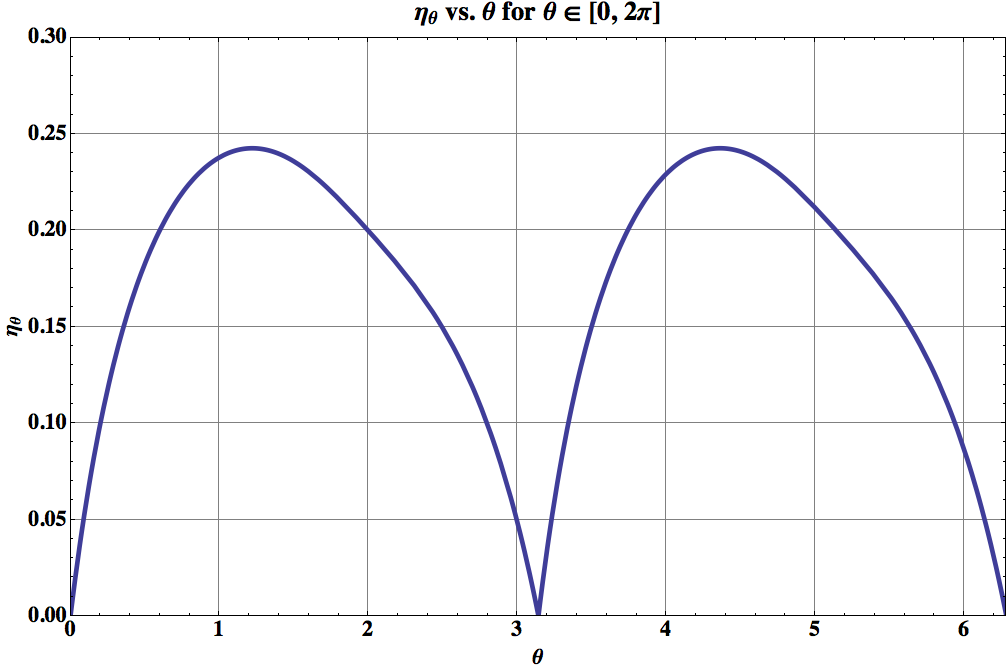
\includegraphics[scale=0.35]{etathetaII.png}
\caption{The negativity $\eta_\theta$ can be plotted as a function of $\theta$ to show the dependency of the negativity on $U_\theta$.  See the text for definitions of $U_\theta$ and $C_\theta$.  The points of vanishing negativity and the periodicity of this plot are also discussed in the text. }
\label{fig:etatheta}
\end{figure}

The negativity $\eta_\theta$ is a function of $\theta$ and can, in principle, be used to gain information about $\theta$.  The negativity can be measured and if the above theoretical definition of the channel is assumed to be true, then $\theta$ can simply be read off Fig.\ \ref{fig:etatheta}.  The negativity $\eta_\theta$ is measured in a single qubit tomography experiment, but $U_\theta$ cannot be directly measured in any such experiment because the composite system contains a qubit defined to be beyond the reach of the experimenter (i.e.\ the bath qubit).   

\subsection{Correlation Alone}
Consider a similar, but different, example:  The new composite dynamics are defined by the controlled phase gate, i.e.\
$$
CZ = \begin{pmatrix}
1&0&0&0\\
0&1&0&0\\
0&0&1&0\\
0&0&0&-1
\end{pmatrix} 
$$
and the sharp operation is defined on the canonical tomography vector $\vec{\tau}$ as
$$
\vec{\tau}^{\sharp_\alpha} = \vec{\tau}\otimes\left(U_\alpha:\vec{\tau}:U_\alpha^\dagger\right)
$$
with
$$
U_\alpha = \alpha\sigma_1 + \sqrt{\left(1-\alpha^2\right)}\sigma_3\;\;,
$$
where $\vec{\sigma}=(\sigma_0,\sigma_1,\sigma_2,\sigma_3)$ is the standard Pauli vector discussed in the tomography section (Sec.\ \ref{sec:tomo}).  Notice, $U_\alpha$ is unitary if $\alpha\in[0,1]$ with $U_\alpha = H_d$ if $\alpha = 2^{-1/2}$.  The Choi representation of a single qubit channel in this two qubit composite system would be
\begin{eqnarray*}
C_\alpha &=& \mathbf{C}\odot\left(CZ:\vec{\tau}^{\sharp_\alpha}:CZ^\dagger\right)^\flat\\
&=& \begin{pmatrix}
 1 & 0 & 0 & \alpha \sqrt{1-\alpha^2} \\
 0 & 0 & \alpha \sqrt{1-\alpha^2} & 0 \\
 0 & \alpha \sqrt{1-\alpha^2} & 0 & 0 \\
 \alpha \sqrt{1-\alpha^2} & 0 & 0 & 1
\end{pmatrix}
\end{eqnarray*}

The spectrum of $C_\alpha$ can be written down immediately as
$$
\operatorname{spec}(C_\alpha) = \{1-x_\alpha,-x_\alpha,x_\alpha,1+x_\alpha\}
$$
where $x_\alpha = \alpha \sqrt{1-\alpha^2}$.  The negativity of this channel $\eta_\alpha$ is bounded by
$$
\alpha\in[0,1]\Rightarrow \eta_\alpha\in\left[0,\frac{1}{6}\right]\;\;,
$$
with $\eta_\alpha=0$ if $\alpha=0$ or $\alpha=1$ and $\eta_\alpha=1/6$ if $\alpha=2^{-1/2}$.  The negativity $\eta_\alpha$ was already calculated for the case when $U_\alpha=H_d$ (i.e.\ $\alpha=2^{-1/2}$) in the discussion of proposed experiments to measure negativity (see Sec.\ \ref{sec:CZprop}).

The dependence of $\eta_\alpha$ on $\alpha$ can plotted to illustrate this idea a little more clearly (see Fig.\ \ref{fig:etaalpha}).     
\begin{figure}[h!t]
\centering
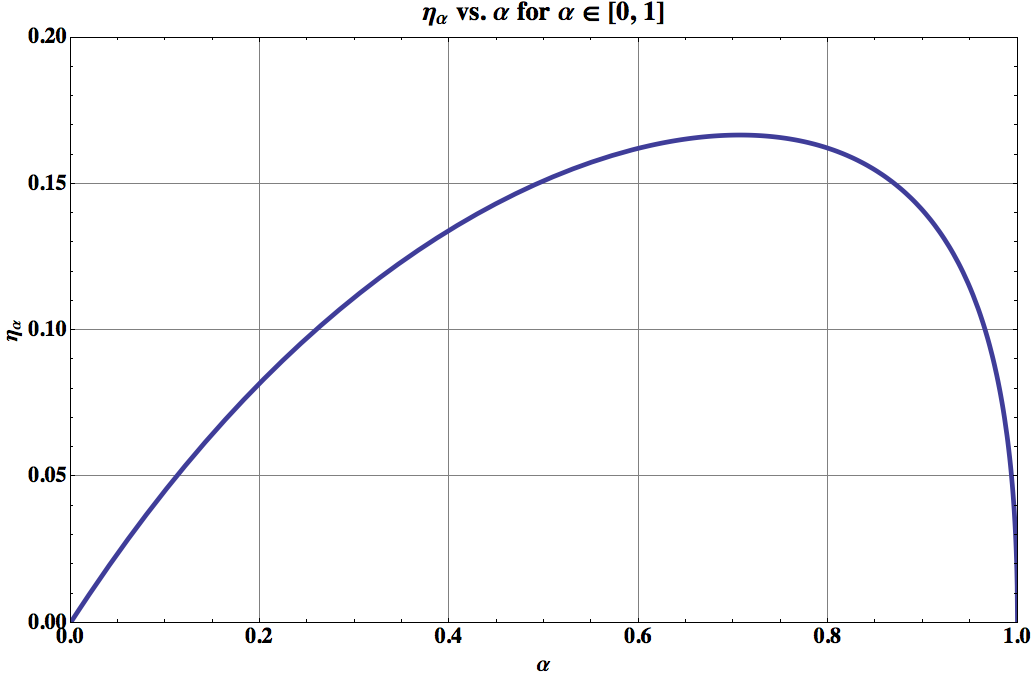
\includegraphics[scale=0.35]{etaalphaII.png}
\caption{The negativity $\eta_\alpha$ can be plotted as a function of $\alpha$ to show the dependency of the negativity on $U_\alpha$.  This example, like the example plotted in Fig.\ \ref{fig:etatheta}, illustrates how the negativity yields information about parameters in the channel definition.}
\label{fig:etaalpha}
\end{figure}   

Again, the negativity $\eta_\alpha$ can be measured and if the above theoretical definition of the channel is assumed to be true, then $\alpha$ can simply be read off Fig.\ \ref{fig:etaalpha}.  In this example, as in the previous one, measurement of the negativity in a tomography experiment grants the experimenter knowledge about channel parameters that cannot be measured directly.  It has been argued that plotting the spectrum of the Choi representation yields information similar to the negativity \cite{Rodriguez2008}, which is true, but the spectrum can become large for multi-qubit channels and the relationship between the eigenvalues (e.g.\ the trace condition of the Choi representation) makes some of the information in the spectrum redundant.  The negativity is meant to be a measure of the system-bath coupling and correlation that condenses information from a tomography experiment into a single parameter, allowing it to be useful (and manageable) beyond the single qubit examples given here.

The above examples are artificial in the sense of comparing the experimentally measured negativity to some known analytical definition of the channel (i.e.\ $C_\theta$ and $C_\alpha$).  Typically, the experimenter will not have very detailed expectations about the form of the channel in the tomography experiment.  Some assumptions might be made about the form of the sharp operation or composite dynamics, but it is rare to have a model of the channel complete enough (or which the experimenter has enough confidence in) to do the type of direct comparison between theory and experiment described in the examples.  Typically, the experimenter would be doing tomography experiments precisely to figure out which assumptions about the sharp and composite dynamics are reasonable.  Nevertheless, even without precise, confidence-worthy models of the experimental channels, measurement of the negativity will provide information about the composite system.  A good example of this point is the experiment conducted in \cite{Cory2004}, which has already been discussed in Sec.\ \ref{sec:Havel}, where the authors used the negativity (which they called the ``positivity'') to try to determine possible problems with their experimental setup. 

\subsection{Coupling and Correlation Together}
Consider a slightly more complicated example with the composite dynamics given by $U_\theta$ and the sharp operation from the above example, i.e. consider the channel\
$$
\varepsilon(\vec{\tau}) = \left(U_\theta:\vec{\tau}^{\sharp_\alpha}:U_\theta^\dagger\right)^\flat\;\;.
$$
This single qubit channel combines the two above examples and will yield a negativity dependent on both the ``correlation'' (i.e.\ $\alpha$) and the ``coupling'' (i.e.\ $\theta$).  The Choi representation of this channel is
\begin{eqnarray*}
C_{\theta\alpha} &=& \mathbf{C}\odot \varepsilon(\vec{\tau})\\
 &=& \begin{pmatrix}
 A & B \\
 B^\dagger & C 
\end{pmatrix}\;\;,
\end{eqnarray*}
where 
$$
A = \begin{pmatrix}
 1-\alpha^2+\alpha^2 \cos^2\theta & -\alpha \sqrt{1-\alpha^2} \sin\theta\\
  -\alpha \sqrt{1-\alpha^2} \sin\theta & \alpha^2 \sin^2\theta 
\end{pmatrix}
$$
$$
B = \begin{pmatrix}
c_1 & c_2 \\
(1+i) \alpha \sqrt{1-\alpha^2} \sin\theta & c_3 
\end{pmatrix}\;\;,
$$
and
$$
C = \begin{pmatrix}
 \alpha^2 \sin^2\theta & -\alpha \sqrt{1-\alpha^2} \sin\theta \\
 -\alpha \sqrt{1-\alpha^2} \sin\theta & 1-\alpha^2+\alpha^2 \cos^2\theta
\end{pmatrix}
$$
with
\begin{eqnarray*}
c_1 &=& \frac{1}{2} \sin\theta \left(\left((-1-i)+2 \alpha^2\right) \cos\theta+2 \alpha \sqrt{1-\alpha^2} \sin\theta\right)\;\;,\\
c_2 &=& \cos\theta+(1+i) \alpha \sqrt{1-\alpha^2} \sin\theta\;\;,
\end{eqnarray*}
and
$$
c_3 = \frac{1}{2} \left((1+i) \cos\theta \sin\theta-2 \alpha^2 \cos\theta \sin\theta-2 \alpha \sqrt{1-\alpha^2} \sin^2\theta\right)\;\;.
$$
Notice $\theta=0$ and $\theta=2\pi$ yield
$$
C_{0\alpha} = C_{2\pi\alpha} = \begin{pmatrix}
 1&0&0&1\\
 0&0&0&0\\
 0&0&0&0\\
 1&0&0&1
\end{pmatrix}
$$  
and $\theta=\pi$ yields
$$
C_{\pi\alpha} = \begin{pmatrix}
 1&0&0&-1\\
 0&0&0&0\\
 0&0&0&0\\
 -1&0&0&1
\end{pmatrix}\;\;.
$$ 
All of these Choi representations $C_{0\alpha}$, $C_{2\pi\alpha}$, and $C_{\pi\alpha}$ represent channels with vanishing negativities independent of the value of $\alpha$.  Notice also that the periodicity of $U_\theta$ is still expected to lead to periodicity in the negativity for this example.  The composite dynamics cyclically have a local unitary form (as was explained in the first example), and local unitary composite dynamics lead to a vanishing negativity for any sharp operation, i.e.\ independent of $\alpha$.  So, there will be periodicity about the point $\theta=\pi$ in this example just an there was in the first example.

The negativity of the channel represented by $C_{\theta\alpha}$ can be plotted as a function of the full two parameter space as a contour map (see Fig.\ \ref{fig:etathetaalpha}).  The negativity can also be plotted as a surface in this two dimensional parameter space, which is done in Fig.\ \ref{fig:etathetaalphaAlso} for a single period of $\theta$ (i.e.\ for $\theta\in[0,\pi]$).
\begin{figure}[h!t]
\centering
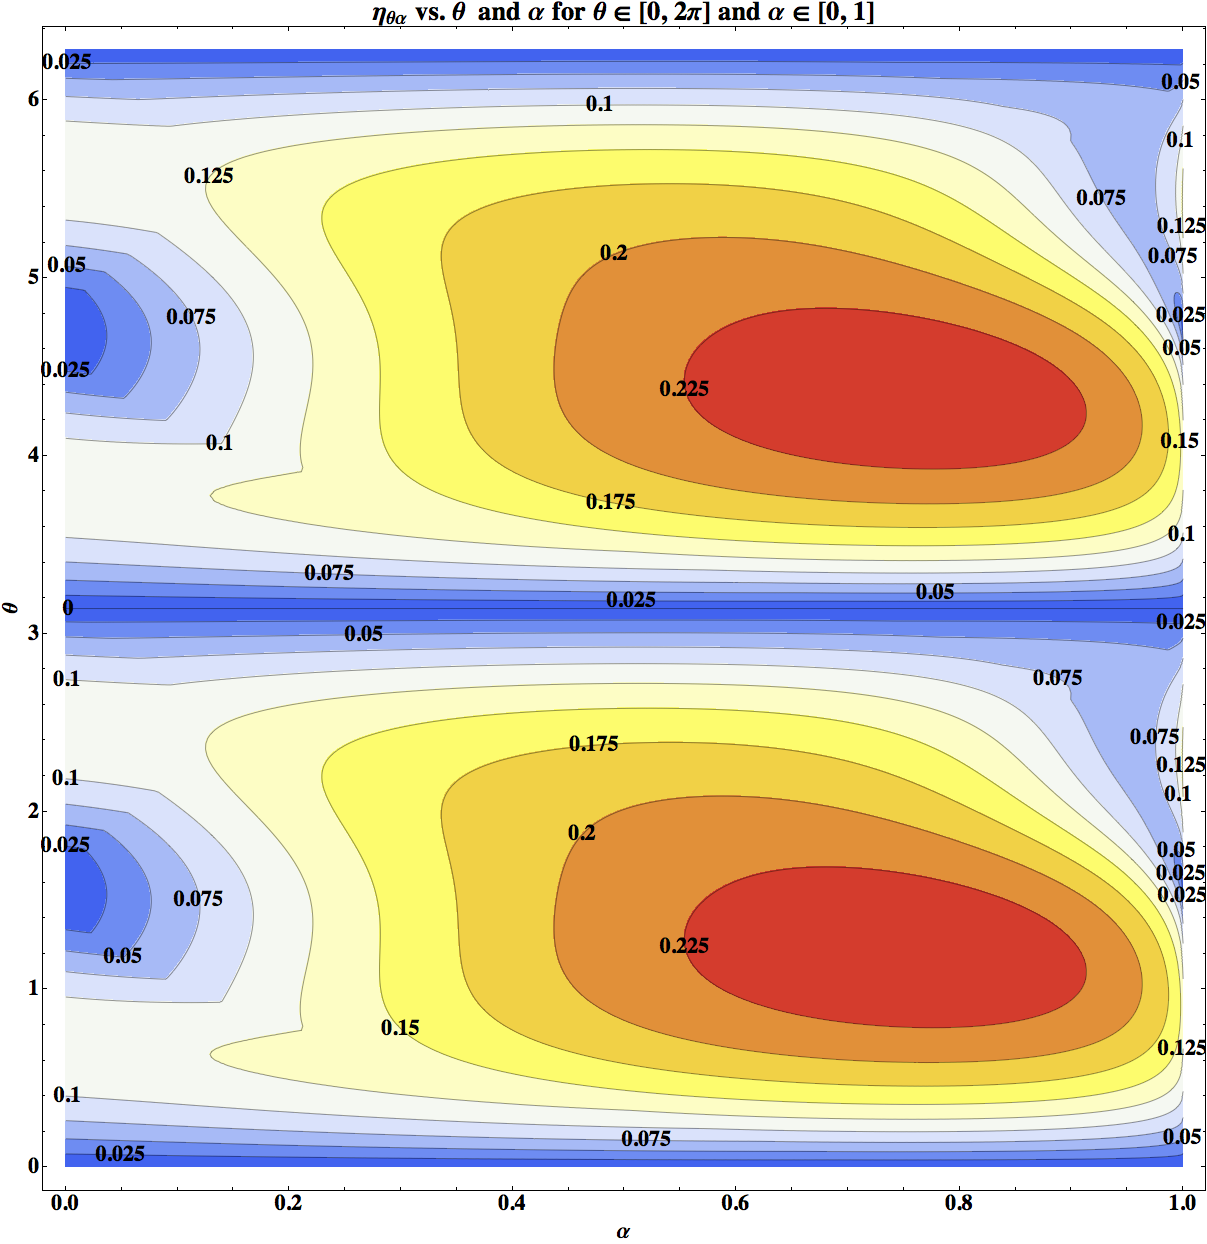
\includegraphics[scale=0.32]{eatthetaalphaII.png}
\caption{The negativity $\eta_{\theta\alpha}$ can be plotted as a function of $\theta$ and $\alpha$ to show the dependency of the negativity on both the correlation and coupling in the channel.  The contours are labeled with the values of the negativity $\eta_{\theta\alpha}$.  The maximum negativity is achieved in the red area of the plot and the minimum is achieved in the blue area of the plot.  See the text for precise definitions of ``correlation'' and ``coupling''. }
\label{fig:etathetaalphaAlso}
\end{figure}
\begin{figure}[t!h]
\centering
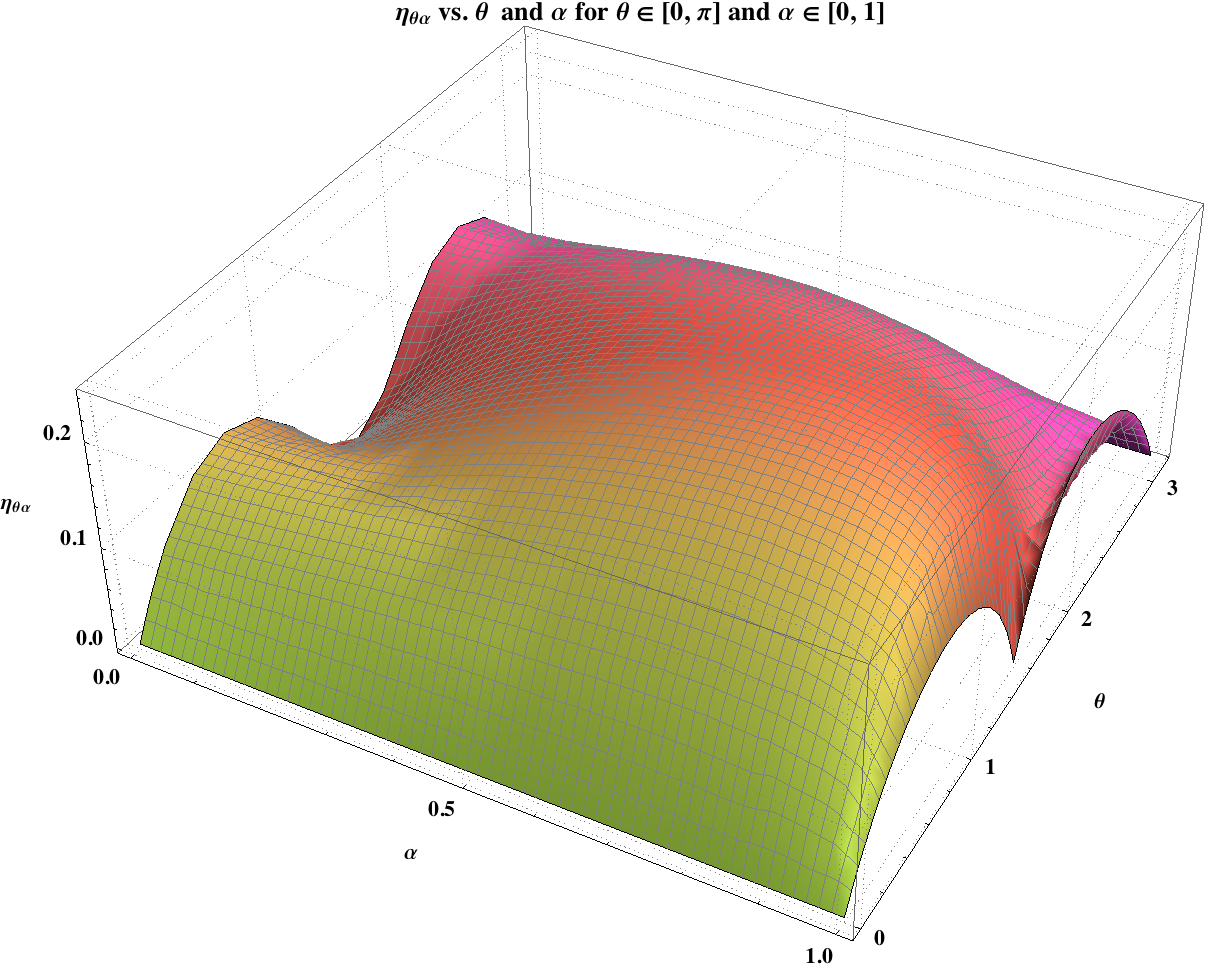
\includegraphics[scale=0.32]{eatthetaalphaIII.png}
\caption{The negativity $\eta_{\theta\alpha}$ can be plotted as a surface in the parameter space of $\theta$ and $\alpha$ to better show the dependency of the negativity on both the correlation and coupling in the channel.  This plot is the surface plot of one period of $\theta$ shown in the contour plot of Fig.\ \ref{fig:etathetaalpha}.}
\label{fig:etathetaalpha}
\end{figure}

The measured value $\eta_{\theta\alpha}$ cannot uniquely identify a location in the two dimensional parameter space plotted in Fig.\ \ref{fig:etathetaalpha}, and this inability is precisely the frustrating limitation of the bath information hidden in the negativity value.  

If the experimenter were able to measure both the negativity and the initial system-bath correlation, then the experimenter would still not be able to draw any conclusions about the causal relationship between the two because the negativity would still be influenced by the unknown coupling.  If he were able to measure the negativity and the coupling, then the system-bath correlation would act in the same manner.  In most situations, the experimenter will only be able to measure the negativity and will be unable to understand the causal relationship between those measurements and the preparation procedure (i.e.\ the correlation) or the composite dynamics (i.e.\ the coupling), unless he is able to control for the relationship between them.   

Notice that the measured negativity will limit the possible values of $\theta$ and $\alpha$ to some subset of the total parameter space which may be substantially smaller and might be helpful to the experimenter.  For example, if the experimenter is attempting to use the measured negativity to develop an empirical model of the coupling and correlation, then this smaller parameter space may make the task of comparing numerical simulations to measured data easier.

\subsection{Determining the Completely Positive Parameter Space}

Consider a ``controlled bath'' type experiment implemented in the lab using the polarization of two maximally entangled photons as qubits.  One photon would act as the reduced system and the other as the bath.  It would be possible to implement the sharp operation presented in Section \ref{sec:couplingalone} as a projective measurement on the reduced system photon after applying a rotation to the bath qubit photon.  The negativity could then be plotted as a function of time.  Repeating this experiment multiple times with different initial rotation angles for the bath qubit would indicate to the experimenter when the composite dynamics are described by local unitaries.  As such, empirically determining when the negativity is zero for a large number of different initial system-bath correlations will allow the experimenter to be reasonably confident of when the composite dynamics are described by local unitaries.  It follows that an experiment that measures the changes in negativity over time for several different initial rotation angles of the bath (i.e.\ $\phi$) can be used to determine when the composite dynamics are in local unitary form without ever knowing anything about the bath dynamics directly.  Such ``controlled bath'' experiments could also be used to understand preparation procedures.
 
These are specific examples of the most straightforward usefulness of the negativity, mapping the completely positive parameter space.  For example, many of the example channels already shown have a Choi representation that takes the form
$$
\mathbf{C} = \begin{pmatrix}
1&0&0&x\\
0&0&y&0\\
0&y^*&0&0\\
x^*&0&0&1
 \end{pmatrix}\;\;.
$$
The spectrum of $\mathbf{C}$ can be written down as 
$$
\operatorname{spec}\left(\mathbf{C}\right) = \left( 1-\sqrt{xx^*},1+\sqrt{xx^*},-\sqrt{yy^*},\sqrt{yy^*}\right)\;\;.
 $$
Notice that $yy^*=0$ and $xx^*\le 1$ are sufficient conditions for this channel to have a vanishing negativity.  These conditions will only be met at specific points in the parameter space of the experiment.  This idea can be illustrated by plotting a few points of vanishing negativity in the 3-dimensional parameter space of $(k_z,t,\phi)$ for the Rabi channel of Section \ref{sec:rabinocoup} (see Fig.\ \ref{fig:CPspace}).  The assumption of a fixed (Hadamard) rotation in the sharp operation of Section \ref{sec:rabinocoup} has been dropped to produce this plot.  Also notice that the planes $t=0$ and $k_z=0$ are not plotted because $t=0$ leads to trivial composite dynamics and $k_z=0$ leads to local unitary composite dynamics.  Both situations imply complete positivity and would clutter the plot unnecessarily.  As such, the plot is over the range $\{k_z,t,\phi\}\in(0,2\pi]$.
 
\begin{figure}[th]
\centering
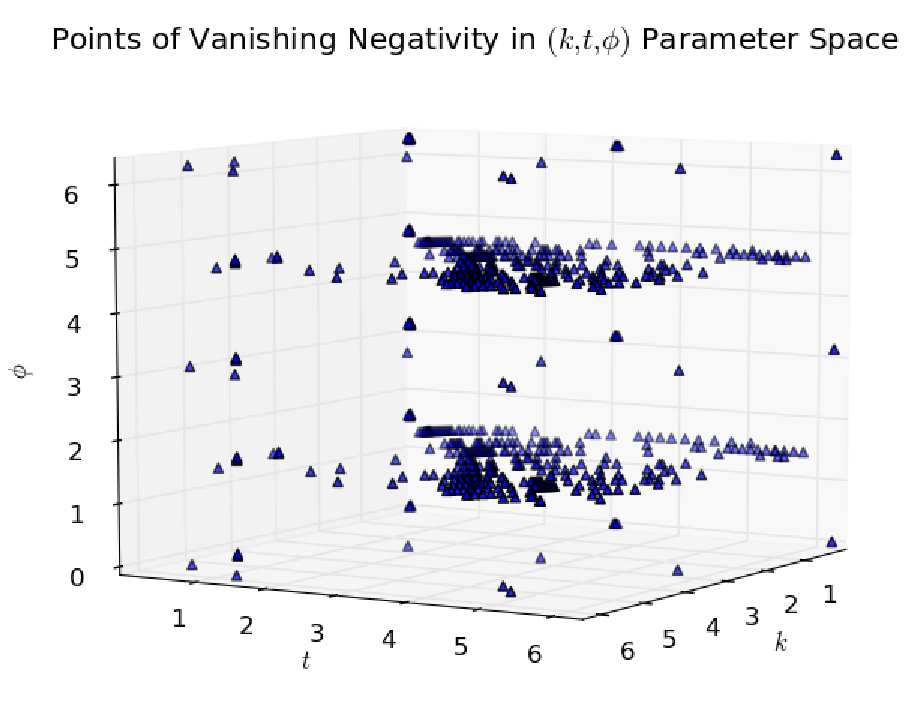
\includegraphics[scale=0.70]{figure9.pdf}
\caption{The points where the negativity of the channel described in Section \ref{sec:rabi} are zero in the parameter space of time $t$, coupling constant $k_z$, and the initial rotation angle of the bath qubit $\phi$.  This plot is meant to illustrate the idea of mapping out a completely positive parameter space.}
 \label{fig:CPspace}
\end{figure} 

\section{Speculation on Utilities}

The ``controlled bath'' situation described in the previous subsection allows the experimenter to circumvent the correlation-coupling delineation problem in the negativity measurement.  If the correlation is precisely controlled, then the negativity can be related directly to the coupling.  The inverse is also true: if an experimenter precisely knows the composite dynamics implemented in a ``controlled bath'' experiment, then the negativity can be related directly to the correlation.  Such an experiment might be used to study preparation procedures or measure correlations in multi-qubit initial states.  

The utility of the negativity is apparent in ``controlled bath'' experiments because these situations are precisely the situations which lend the negativity a straightforward relationship with the bath.  The negativity, however, may be useful beyond these experiments.  The negativity provides information about the bath.  The bath is defined by the experimenter's ignorance.  Hence, the negativity provides information about part of the quantum system traditionally considered unknowable.  The inscrutable effects of the bath through the coupling and correlation can be observed through negativity measurements.  Such information is academically interesting and might have practical use in engineering quantum technologies and/or understanding the limitations of those technologies.  A channel with a non-zero negativity has some correlation or coupling (or both) with the bath and such interactions with the bath might lead to new understanding of the information theoretic properties of quantum channels.  For example, such channels might have different capacities than their completely positive counter parts, or the security of such channels might not be understood in the same way.


